\documentclass[11pt, a4paper]{article}

% --- PACKAGES ---
\usepackage[margin=1in]{geometry}
\usepackage{amsmath}
\usepackage{graphicx}
\usepackage{booktabs} % For professional tables
\usepackage{amssymb} % For symbols like \mathbb{R}
\usepackage{amsfonts}
\usepackage{bm} % For bold math symbols
\usepackage{amsthm} % For theorem-like environments
\usepackage{enumitem} % For customized lists
\usepackage{tabularx}
\usepackage{ragged2e}
\usepackage[utf8]{inputenc}
\usepackage{tabularx}
\usepackage{booktabs}
\usepackage{amsmath}
\usepackage{geometry}
\usepackage{listings}
\usepackage{xcolor}
% --- DOCUMENT SETUP ---
% We define the title elements manually inside the 'titlepage' environment
% \title{Technical Reference Note: \\ A Modern Framework for Smoothing in Additive Models}
% \author{Personal Reference Document}
% \date{\today}

\newtheorem{definition}{Definition}
\newtheorem{theorem}{Theorem}
\newtheorem{lemma}{Lemma}
% R code styling
\lstset{
    language=R,
    basicstyle=\ttfamily\small,
    keywordstyle=\color{blue},
    commentstyle=\color{gray},
    stringstyle=\color{red},
    numbers=left,
    numberstyle=\tiny,
    stepnumber=1,
    numbersep=5pt,
    backgroundcolor=\color{gray!10},
    frame=single,
    breaklines=true,
    breakatwhitespace=false,
    showspaces=false,
    showstringspaces=false,
    showtabs=false,
    tabsize=2
}

% --- BEGIN DOCUMENT ---
\begin{document}


\begin{titlepage}
 \centering % Center everything on the page
 
 \vspace*{1cm} % Add some space at the top
 
 {\Huge \bfseries Splines Overview}
 
 \vspace{2cm} % Space between title and image
 
 % --- IMAGE ---
 % Make sure the image file 'spline-ducks.png' is in the same directory
 % as your .tex file. Adjust width as needed.
 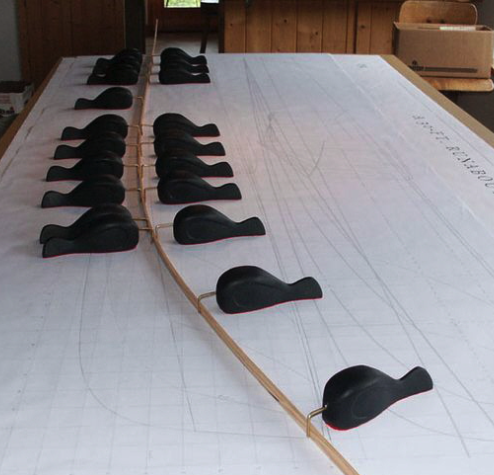
\includegraphics[width=0.6\linewidth]{spline-ducks.png}
 
 \vfill % Pushes the content below to the bottom of the page
  
 \vspace{1cm}
 
 {\large \today}

\end{titlepage}

\tableofcontents
\newpage
\section{Intro to Splines and Smoothing}
\subsection{1.1 The Physical Analogy: The Draftsman's Spline}
The term ``spline'' originates from a tool used by draftsmen: a long, thin, flexible strip of wood. To draw a smooth curve through a set of points, they would place lead weights (``ducks'') at the required locations and bend the strip against them. The strip naturally settles into a shape that minimizes its total bending energy. This physical concept is mathematically equivalent to minimizing the integrated squared second derivative of a function, $\int [f''(x)]^2 dx$, which is a measure of its total ``wiggliness''.


\subsection{1.2 Basis Functions}
Instead of defining a single complex function, we can construct it from a set of simple, known ``building block'' of functions, $b_k(x)$, called a \textbf{basis}. The final complex curve $f(x)$ is a weighted sum of these blocks:
\[ f(x) = \sum_{k=1}^{K} \beta_k b_k(x) \]
The smoothness of $f(x)$ is determined by the values of the coefficients $\beta_k$. If adjacent coefficients are very different, the curve will be wiggly. If they are similar, it will be smooth. ``Penalizing wiggliness'' therefore becomes equivalent to penalizing large differences between adjacent coefficients.
\begin{figure}[h!]
 \centering
 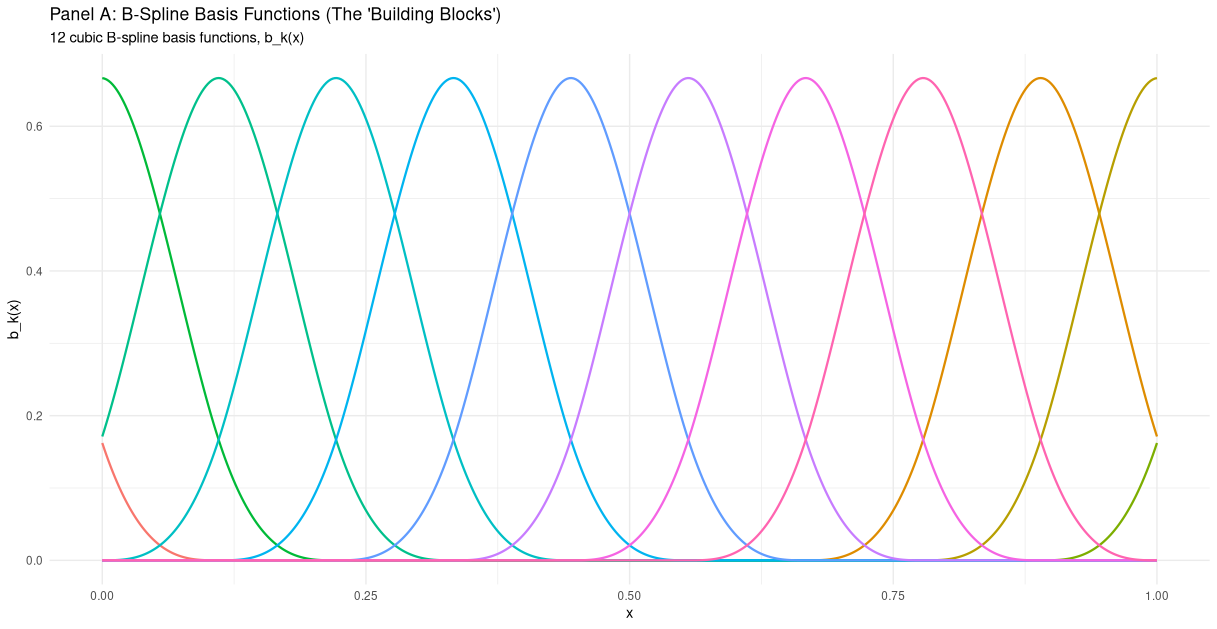
\includegraphics[width=\linewidth]{b-splines.png}
 \caption{B Spline Basis Functions}
 \label{fig:enter-label-1}
\end{figure}

\begin{figure}[h!]
 \centering
 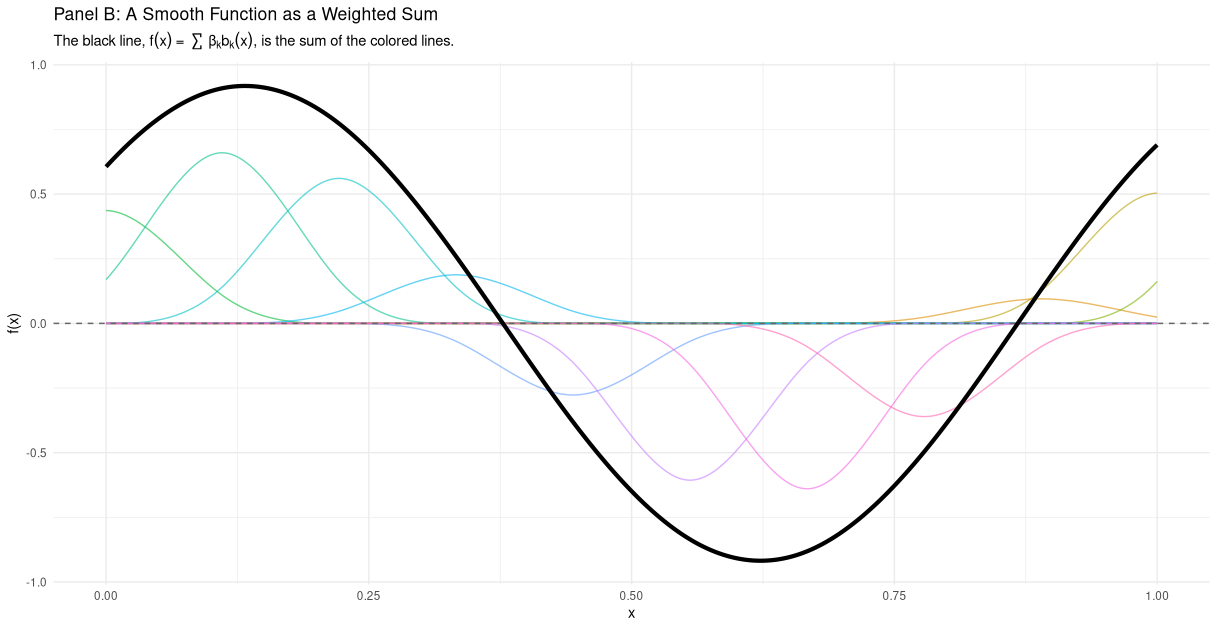
\includegraphics[width=1\linewidth]{weighted.png}
 \caption{Weighted Basis Functions}
 \label{fig:enter-label-2}
\end{figure}

\newpage
\section{Knot placement and Penalized Splines}
The development of penalized splines was largely motivated by the inherent difficulties encountered with earlier spline methodologies, particularly concerning the selection of knots and the risk of overfitting when using flexible basis expansions. 

\subsection{2.1 The Limitations of Manual Knot Placement: Subjectivity, Misspecification, and Instability}
In traditional spline regression, the function is constructed by joining polynomial pieces at specific points known as knots. The number and location of these knots are critical as they dictate the flexibility of the spline. If too few knots are used, the spline may be too stiff to capture the true underlying function $\Rightarrow $ underfitting. Conversely, while more knots offer greater flexibility, their improper placement or an excessive number in an unpenalized setting can lead to overfitting.

Manual selection of knots introduces several significant limitations:
\begin{itemize}
 \item \textbf{Subjectivity and Reproducibility:} The choice of knot locations is often subjective, relying on visual inspection of the data or domain expertise. Different analysts, or even the same analyst at different times, might select different knot configurations for the identical dataset. This subjectivity inherently compromises the reproducibility of the model and its findings, which is a fundamental tenet of scientific research. While the goal of employing splines is often to allow the data to determine the functional form without strong parametric assumptions, manual knot selection reintroduces a substantial element of user judgment.

 \item \textbf{Misspecification Bias:} If knots are not placed in regions where the true underlying function exhibits changes in behavior—such as peaks, troughs, or points of inflection—the spline will be unable to adapt to these features adequately. This leads to misspecification bias, where the fitted model systematically deviates from the true function in those regions. For instance, if a function has a sharp peak but no knot is placed near it, the spline will smooth over this feature. The performance of splines is highly dependent on the chosen knot locations. Improper placement can lead to a misrepresentation of the data's inherent structure.

 \item \textbf{Underfitting:} A common issue arising from manual selection is the use of too few knots. This results in a spline that is overly stiff and lacks the necessary flexibility to capture the true complexity present in the data, leading to underfitting. Visualizing this, attempting to fit a complex, oscillating function with only a few knots will inevitably result in a poor representation that misses key variations.

 \item \textbf{Local Overfitting and Instability:} Even if a seemingly reasonable number of knots is chosen, their suboptimal placement can be problematic. For example, clustering knots in relatively flat regions of the function while having too few knots in highly variable (wiggly) regions can lead to the spline fitting noise locally in the over-parameterized segments and underfitting in others. This can result in an unstable overall fit. The sensitivity to knot choices is well-documented; for instance, increasing the number of knots or repeating knots directly impacts the smoothness and local behavior of the spline fit.

 \item \textbf{"Optimal" Knot Placement:} Recognizing these difficulties, considerable research effort was historically dedicated to developing methods for automatically selecting "optimal" knot points. Techniques such as Generalized Cross-Validation (GCV), Akaike's Information Criterion (AIC), or Bayesian Information Criterion (BIC) were employed to guide knot selection. Strategies included placing knots at quantiles of the predictor variable or using domain-specific knowledge. While these automated methods were an improvement over purely manual selection, they often involved significant computational burden, especially if cross-validation was performed over many potential knot sets. Furthermore, they did not fully resolve the issue of pre-specifying the \textbf{number} of knots, which itself influences the optimal locations. 
\end{itemize}
The challenges associated with manual or heuristic knot selection—subjectivity, potential for misspecification and underfitting, and the computational cost of optimization—were significant drivers for the development of penalized spline methods. These modern approaches aim to make the choice of knots, particularly their number and exact locations, far less critical by employing a different strategy: using a sufficiently large number of knots and controlling the model's smoothness via a penalty term.

\subsection{2.2  Overfitting  of  Unpenalized Basis Functions}
To circumvent the difficulties of selecting a small, optimal set of knots, an alternative approach might be to use a very large number of basis functions. This implies using many knots, often placed at regular intervals across the range of the covariate, or even, in the limit of classical smoothing splines, a knot at every unique data point. The rationale is to ensure that the basis is rich enough to capture any potential complexity in the underlying function. However, if these basis functions are used in a standard regression framework without any form of regularization (i.e., unpenalized), a severe problem known as overfitting arises.

Consider the standard linear model formulation $\mathbf{y} = \mathbf{X}\boldsymbol{\beta} + \boldsymbol{\epsilon}$, where $\mathbf{y}$ is the vector of observed responses, $\mathbf{X}$ is the $n \times K$ model matrix derived from $K$ basis functions evaluated at $n$ observation points, $\boldsymbol{\beta}$ is the vector of $K$ coefficients to be estimated, and $\boldsymbol{\epsilon}$ is the vector of random errors. If $K$ is large, potentially approaching or exceeding $n$, this becomes a high-dimensional regression problem.

\begin{itemize}
 \item \textbf{Fitting Noise Instead of Signal:} With a large number of coefficients $\beta_k$, an unpenalized model possesses excessive flexibility. This flexibility allows the model to fit not only the underlying systematic relationship between the covariates and the response but also the random noise $\boldsymbol{\epsilon}$ present in the training data. The resulting fitted curve will contort itself to pass very close to, or even exactly through, the observed data points, including their random fluctuations. Visual examples demonstrate that a spline with many knots and no penalty becomes "extremely wiggly" and is clearly not a good representation of the true, smoother underlying function. This phenomenon is akin to an interpolating spline when the number of effective parameters matches the number of unique data points; while interpolation serves specific purposes, it is generally undesirable for statistical modeling of noisy data as it perfectly reproduces the noise component.

 \item \textbf{Poor Generalization Performance:} A model that has meticulously fitted the noise in the training data will exhibit excellent performance on that same data (e.g., a very high $R^2$ or very low sum of squared errors). However, it will generalize poorly to new, unseen data. The specific patterns of noise learned from one dataset are unlikely to be replicated in another. Consequently, the overfitted model's predictions on new data will have high variance.
\end{itemize}
 \begin{figure}[h!]
  \centering
  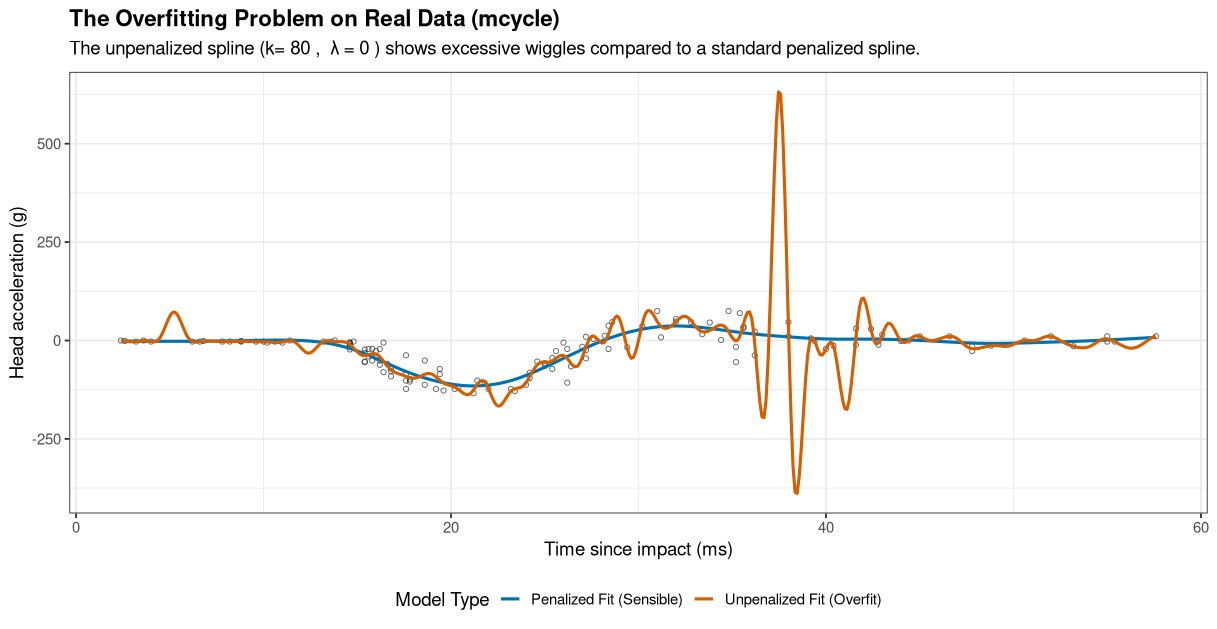
\includegraphics[width=\linewidth]{overfit.png}
  \caption{Overfitted spline}
  \label{fig:enter-label-3}
 \end{figure}
\subsection{2.3 Penalized Splines – A Principled Approach to Smoothness}
The  framework of penalized splines offers an elegant resolution to the twin problems of knot selection and overfitting. The core idea is to begin with a basis that is rich enough to represent complex functions—typically involving a generous number of knots that are often, though not necessarily, evenly spaced—and then to introduce a penalty term into the estimation criterion that explicitly discourages excessive "wiggliness" or complexity in the fitted function. The fitting process then automatically balances fidelity to the data against the smoothness imposed by this penalty.

The coefficients $\boldsymbol{\beta}$ of the basis functions are determined by minimizing a \textbf{penalized least squares objective function}:
\[ \min_{\boldsymbol{\beta}} \left\{ ||\mathbf{y} - \mathbf{X}\boldsymbol{\beta}||^2 + \lambda \boldsymbol{\beta}^T \mathbf{S} \boldsymbol{\beta} \right\} \]
This objective function has two main components:
\begin{enumerate}
 \item $||\mathbf{y} - \mathbf{X}\boldsymbol{\beta}||^2$: This is the standard sum of squared errors (SSE), measuring the goodness-of-fit of the model to the observed data $\mathbf{y}$. Minimizing this term alone would lead to an unpenalized fit, prone to overfitting if the basis $\mathbf{X}$ is rich.
 \item $\lambda \boldsymbol{\beta}^T \mathbf{S} \boldsymbol{\beta}$: This is the \textbf{penalty term} that quantifies the "wiggliness" of the function represented by $\boldsymbol{\beta}$.
 \begin{itemize}
  \item $\lambda \ge 0$ is the \textbf{smoothing parameter}. It is a crucial tuning parameter that controls the trade-off between goodness-of-fit and smoothness.
  \begin{itemize}
\item If $\lambda = 0$, there is no penalty, and the objective reduces to ordinary least squares. If the basis is rich, this can lead to overfitting, where the spline may interpolate the data.[10]
\item As $\lambda \rightarrow \infty$, the penalty term dominates the objective function. To minimize the overall expression, the model is forced to make $\boldsymbol{\beta}^T \mathbf{S} \boldsymbol{\beta}$ very small. This results in a very smooth function. For instance, with a typical second-derivative penalty, the fitted function will approach a straight line (the smoothest possible function in that context).
\item An appropriate, finite, positive value of $\lambda$ achieves a balance, producing a smooth function that captures the underlying trend in the data without fitting the noise. The selection of this optimal $\lambda$ is a key aspect of penalized spline methodology.
  \end{itemize}
  \item $\mathbf{S}$ is the \textbf{penalty matrix}. This $K \times K$ symmetric, positive semi-definite matrix defines precisely what constitutes "wiggliness" in terms of the basis coefficients $\boldsymbol{\beta}$. The structure of $\mathbf{S}$ depends on the chosen basis functions and the type of penalty applied (e.g., penalties based on integrated squared derivatives of $f(x)$ or penalties based on finite differences of the coefficients $\beta_k$). This will be explored in detail in Part 3.
 \end{itemize}
\end{enumerate}
A significant advantage of the penalized spline approach is that the \textbf{choice of knots becomes far less critical} than in classical regression splines. As long as a sufficiently large number of knots are used to span the range of the data and allow for potential complexity, their exact placement is not a primary concern. The smoothness of the resulting function is primarily controlled by the smoothing parameter $\lambda$, not by meticulous knot selection. For instance, a common strategy is to use a number of knots proportional to $\min(n/4, 40)$, often placed at quantiles of the predictor or simply evenly spaced. This "rich basis then constrain" philosophy is a general theme in modern statistical modeling: start with a model class flexible enough to capture complex signals and then use regularization to select a desirable solution from this class.

The penalty term $\lambda \boldsymbol{\beta}^T \mathbf{S} \boldsymbol{\beta}$ can be viewed as a form of shrinkage on the coefficients $\boldsymbol{\beta}$, analogous to ridge regression. However, unlike standard ridge regression where the penalty is $\lambda ||\boldsymbol{\beta}||_2^2 = \lambda \boldsymbol{\beta}^T \mathbf{I} \boldsymbol{\beta}$ (shrinking all coefficients uniformly towards zero), the penalty matrix $\mathbf{S}$ in penalized splines imposes a structured shrinkage. It specifically penalizes combinations of coefficients that lead to functions deemed too "wiggly" according to the definition embodied in $\mathbf{S}$.

\begin{figure}[h!]
 \centering
 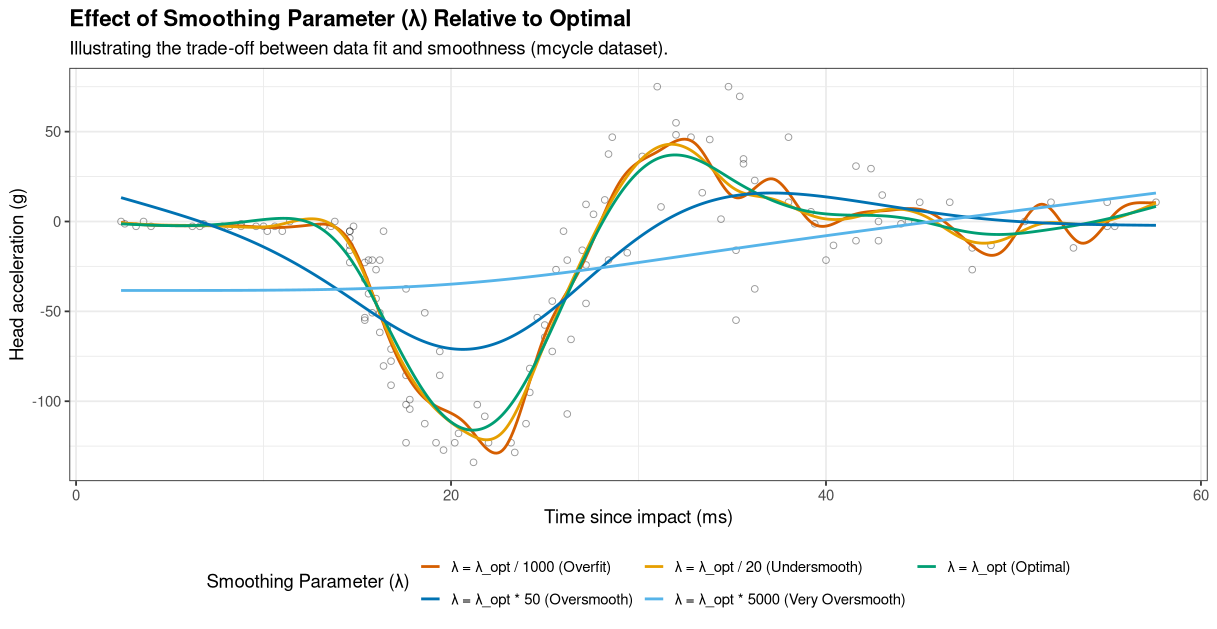
\includegraphics[width=\linewidth]{optimal_over_under.png}
 \caption{Visualisation of different choices of $\lambda$}
 \label{fig:enter-label-4}
\end{figure}

\newpage
\section{ Penalized Spline Components}
Having established the foundational problem and the conceptual solution offered by penalized splines, this section provides a more detailed mathematical examination of the core components: the basis expansion used to represent the smooth function, the construction and interpretation of the wiggliness penalty, the derivation of the penalized least squares solution, and the concept of effective degrees of freedom which quantifies model complexity.

\subsection{3.1 The Basis Expansion and Model Matrix $\mathbf{X}$}
The first step in constructing a penalized spline is to define a set of basis functions, $b_k(x)$, which are combined linearly to approximate the unknown smooth function $f(x)$. The choice of basis functions and their number, $K$, determines the flexibility of the function space within which we are searching for our estimate.

\paragraph{Mathematical Formulation}
The smooth function $f(x)$ is approximated by a linear combination of $K$ basis functions:
\[ f(x) = \sum_{k=1}^{K} \beta_k b_k(x) \]
Here, $b_k(x)$ is the $k$-th basis function, which is a known function of the covariate $x$, and $\beta_k$ is the corresponding coefficient that needs to be estimated from the data. The number of basis functions, $K$, is typically chosen to be sufficiently large to ensure that the basis is flexible enough to capture potentially complex patterns in the data, without being so excessively large as to create undue computational burden. In the penalized spline framework, the exact value of $K$ is less critical than in unpenalized regression splines, as the penalty term will control the effective smoothness.

\paragraph{Commonly Used Basis Functions}
Several types of basis functions are commonly employed in penalized spline models:
\begin{itemize}
 \item \textbf{B-splines:} B-splines are perhaps the most widely used basis functions for penalized splines, particularly for P-splines (discussed in Part 4). They are piecewise polynomial functions of a specified degree (e.g., cubic B-splines, which are piecewise cubic polynomials, are common). A key property of B-splines is their \textit{local support}: each basis function $b_k(x)$ is non-zero only over a limited range of $x$, typically spanning a few knot intervals. This local support leads to banded (sparse) model and penalty matrices, which is computationally advantageous, especially for large $K$. Visualizations of B-spline basis functions often show characteristic "bell-shaped" curves that overlap with their neighbors.

 \item \textbf{Truncated Power Series Basis:} Another way to represent splines is using a truncated power series basis. For a spline of degree $d$ with $M_{knots}$ interior knots $\kappa_1, \dots, \kappa_{M_{knots}}$, this basis consists of the polynomials $1, x, x^2, \dots, x^d$ and the truncated power functions $(x-\kappa_j)_+^d$ for $j=1, \dots, M_{knots}$. The function $(u)_+$ is defined as $u$ if $u > 0$ and $0$ otherwise. While conceptually simple, truncated power series bases can lead to severe numerical instability (ill-conditioning) when $K$ is large, due to high correlation between basis functions. B-splines are generally preferred for their superior numerical properties.

 \item Other bases, such as those derived from the eigenfunctions of differential operators (as in Thin Plate Regression Splines, see Section 4.2), are also used.
\end{itemize}
The choice of basis functions represents a trade-off between numerical stability, computational efficiency for constructing the basis and penalty matrices, and the ease with which certain types of penalties can be imposed.

\paragraph{Constructing the Model Matrix $\mathbf{X}$}
Given $n$ observations $(x_i, y_i)$, $i=1, \dots, n$, the vector of evaluated smooth function values $\mathbf{f} = [f(x_1), f(x_2), \dots, f(x_n)]^T$ can be expressed in matrix form as:
\[ \mathbf{f} = \mathbf{X}\boldsymbol{\beta} \]
where $\boldsymbol{\beta} = [\beta_1, \beta_2, \dots, \beta_K]^T$ is the $K \times 1$ vector of basis coefficients. The $n \times K$ matrix $\mathbf{X}$ is known as the \textbf{model matrix} (or design matrix). Each element $X_{ik}$ of this matrix is the value of the $k$-th basis function $b_k(x)$ evaluated at the $i$-th covariate value $x_i$:
\[ X_{ik} = b_k(x_i) \]
Thus, the $i$-th row of $\mathbf{X}$ is $[b_1(x_i), b_2(x_i), \dots, b_K(x_i)]$, and the $k$-th column is $[b_k(x_1), b_k(x_2), \dots, b_k(x_n)]^T$. The construction of this matrix is a standard procedure in software packages that implement splines; for example, the `splines2` package in R provides functions like `bSpline()` to generate B-spline basis matrices.

The use of a basis expansion effectively transforms the non-parametric problem of estimating an unknown function $f(x)$ into a parametric problem of estimating the coefficients $\boldsymbol{\beta}$, albeit often in a high-dimensional parameter space. This transformation is fundamental, as it allows the application of familiar (penalized) least squares or likelihood-based estimation techniques. The structure of $\mathbf{X}$ (e.g., its sparsity, conditioning) is directly influenced by the choice of basis functions and knot locations, which in turn affects computational efficiency and the numerical stability of the estimation process.

\subsection{3.2 The Wiggliness Penalty: $\lambda \boldsymbol{\beta}^T \mathbf{S} \boldsymbol{\beta}$}
The wiggliness penalty, $\lambda \boldsymbol{\beta}^T \mathbf{S} \boldsymbol{\beta}$, is the component of the penalized least squares objective that controls the smoothness of the fitted function. It quantifies the "roughness" or "complexity" of the function $f(x) = \sum \beta_k b_k(x)$ in terms of its coefficients $\boldsymbol{\beta}$.

\paragraph{Derivation from Integrated Squared Derivatives}
A classical approach to defining the wiggliness of a function $f(x)$ is to measure the energy associated with its derivatives. Commonly, the integral of the squared $m$-th derivative is used:
\[ \text{Penalty Functional} = \int [f^{(m)}(x)]^2 dx \]
For instance, if $m=2$, the penalty is $\int [f''(x)]^2 dx$, which penalizes functions with high curvature (rapidly changing slope), as in the physical analogy of the draftsman's spline.

To express this functional in terms of the basis coefficients $\boldsymbol{\beta}$, we substitute $f(x) = \sum_{k=1}^{K} \beta_k b_k(x)$. The $m$-th derivative is $f^{(m)}(x) = \sum_{k=1}^{K} \beta_k b_k^{(m)}(x)$. Let $\mathbf{b}^{(m)}(x)$ be the $K \times 1$ vector with elements $b_k^{(m)}(x)$. Then $f^{(m)}(x) = \boldsymbol{\beta}^T \mathbf{b}^{(m)}(x) = (\mathbf{b}^{(m)}(x))^T \boldsymbol{\beta}$.
The squared $m$-th derivative is $[f^{(m)}(x)]^2 = (\boldsymbol{\beta}^T \mathbf{b}^{(m)}(x)) ((\mathbf{b}^{(m)}(x))^T \boldsymbol{\beta}) = \boldsymbol{\beta}^T \left( \mathbf{b}^{(m)}(x) (\mathbf{b}^{(m)}(x))^T \right) \boldsymbol{\beta}$.
Integrating this expression yields:
\[ \int [f^{(m)}(x)]^2 dx = \boldsymbol{\beta}^T \left( \int \mathbf{b}^{(m)}(x) (\mathbf{b}^{(m)}(x))^T dx \right) \boldsymbol{\beta} \]
Thus, the penalty matrix $\mathbf{S}$ is a $K \times K$ matrix whose elements are given by:
\[ S_{jk} = \int b_j^{(m)}(x) b_k^{(m)}(x) dx \]
This matrix $\mathbf{S}$ is symmetric and positive semi-definite. The penalty term becomes $\boldsymbol{\beta}^T \mathbf{S} \boldsymbol{\beta}$. For example, if $m=2$, $S_{jk} = \int b_j''(x) b_k''(x) dx$.[21]

\paragraph{P-spline Difference Penalties}
An alternative and computationally convenient approach, popularized by Eilers and Marx (1996) for P-splines, is to define the penalty based on finite differences of adjacent B-spline coefficients. This approximates the integrated derivative penalty but is often simpler to construct.
The rationale is that if the function is smooth, its B-spline coefficients should also form a smooth sequence. Large differences between adjacent coefficients imply rapid changes and thus "wiggliness."
Let $\Delta^m \beta_k$ denote the $m$-th order difference of the coefficients.
\begin{itemize}
 \item First-order difference ($m=1$): $\Delta \beta_k = \beta_k - \beta_{k-1}$ (penalizes jumps in coefficient values).
 \item Second-order difference ($m=2$): $\Delta^2 \beta_k = \Delta(\Delta \beta_k) = (\beta_k - \beta_{k-1}) - (\beta_{k-1} - \beta_{k-2}) = \beta_k - 2\beta_{k-1} + \beta_{k-2}$ (penalizes changes in the slope of the coefficient sequence, i.e., curvature).
\end{itemize}
The penalty is then the sum of squares of these differences: $\sum_{k} (\Delta^m \beta_k)^2$.
This sum can be expressed in matrix form. Let $\mathbf{D}_m$ be a differencing matrix of appropriate dimensions such that the vector of $m$-th differences is $\mathbf{D}_m \boldsymbol{\beta}$. Then the penalty is $(\mathbf{D}_m \boldsymbol{\beta})^T (\mathbf{D}_m \boldsymbol{\beta}) = \boldsymbol{\beta}^T \mathbf{D}_m^T \mathbf{D}_m \boldsymbol{\beta}$.
In this case, the penalty matrix is $\mathbf{S} = \mathbf{D}_m^T \mathbf{D}_m$.[17, 23]

For example, with $K$ coefficients:
\begin{itemize}
 \item For $m=1$, $\mathbf{D}_1$ is a $(K-1) \times K$ matrix:
 \[ \mathbf{D}_1 = \begin{pmatrix} -1 & 1 & 0 & \dots & 0 \\ 0 & -1 & 1 & \dots & 0 \\ \vdots & & \ddots & & \vdots \\ 0 & \dots & 0 & -1 & 1 \end{pmatrix} \]
 \item For $m=2$, $\mathbf{D}_2$ is a $(K-2) \times K$ matrix:
 \[ \mathbf{D}_2 = \begin{pmatrix} 1 & -2 & 1 & 0 & \dots & 0 \\ 0 & 1 & -2 & 1 & \dots & 0 \\ \vdots & & \ddots & & & \vdots \\ 0 & \dots & 0 & 1 & -2 & 1 \end{pmatrix} \]
 \item For $m=3$, $\mathbf{D}_3$ is a $(K-3) \times K$ matrix:
 \[ \mathbf{D}_3 = \begin{pmatrix} -1 & 3 & -3 & 1 & 0 & \dots & 0 \\ 0 & -1 & 3 & -3 & 1 & \dots & 0 \\ \vdots & & \ddots & & & & \vdots \\ 0 & \dots & 0 & -1 & 3 & -3 & 1 \end{pmatrix} \]
\end{itemize}
The choice of the order $m$ for the penalty reflects an implicit assumption about the nature of the function's smoothness. A second-order penalty ($m=2$) is very common, as it penalizes deviations from local linearity in the function (or its coefficients) and leads to visually smooth curves. The sparsity of $\mathbf{D}_m$ (it is a banded matrix) means that $\mathbf{S}=\mathbf{D}_m^T\mathbf{D}_m$ is also banded and sparse, which is computationally very efficient.

\paragraph{The Smoothing Parameter $\lambda$}
The scalar $\lambda \ge 0$ multiplies the entire penalty term $\boldsymbol{\beta}^T \mathbf{S} \boldsymbol{\beta}$. It governs the strength of the penalty and thus controls the trade-off between fitting the data closely and maintaining smoothness. A larger $\lambda$ imposes a heavier penalty on wiggliness, leading to a smoother function, while a smaller $\lambda$ allows the function to be more flexible and fit the data more closely. The selection of $\lambda$ is a critical aspect of penalized spline modeling and will be discussed further in Part 5.

The penalty term, by adding a regularization constraint, transforms what could be an ill-posed problem (fitting an overly flexible model to noisy data) into a well-posed one, ensuring a unique and stable solution.

\subsection{3.3 The Penalized Least Squares Solution $\hat{\boldsymbol{\beta}}$ and Influence Matrix $\mathbf{A}$}
The coefficients $\hat{\boldsymbol{\beta}}$ for the penalized spline are found by minimizing the penalized least squares objective function:
\[ L(\boldsymbol{\beta}) = ||\mathbf{y} - \mathbf{X}\boldsymbol{\beta}||^2 + \lambda \boldsymbol{\beta}^T \mathbf{S} \boldsymbol{\beta} \]
This is a quadratic function of $\boldsymbol{\beta}$, and its minimum can be found by setting its derivative with respect to $\boldsymbol{\beta}$ to zero.

\paragraph{Derivation of $\hat{\boldsymbol{\beta}}$}
The objective function can be expanded as:
\[ L(\boldsymbol{\beta}) = (\mathbf{y} - \mathbf{X}\boldsymbol{\beta})^T(\mathbf{y} - \mathbf{X}\boldsymbol{\beta}) + \lambda \boldsymbol{\beta}^T \mathbf{S} \boldsymbol{\beta} \]
\[ L(\boldsymbol{\beta}) = \mathbf{y}^T\mathbf{y} - \mathbf{y}^T\mathbf{X}\boldsymbol{\beta} - \boldsymbol{\beta}^T\mathbf{X}^T\mathbf{y} + \boldsymbol{\beta}^T\mathbf{X}^T\mathbf{X}\boldsymbol{\beta} + \lambda \boldsymbol{\beta}^T \mathbf{S} \boldsymbol{\beta} \]
Since $\mathbf{y}^T\mathbf{X}\boldsymbol{\beta}$ is a scalar, it is equal to its transpose $\boldsymbol{\beta}^T\mathbf{X}^T\mathbf{y}$. Assuming $\mathbf{S}$ is symmetric (which is standard for penalty matrices derived from squared derivatives or difference operators), we have:
\[ L(\boldsymbol{\beta}) = \mathbf{y}^T\mathbf{y} - 2\boldsymbol{\beta}^T\mathbf{X}^T\mathbf{y} + \boldsymbol{\beta}^T(\mathbf{X}^T\mathbf{X} + \lambda\mathbf{S})\boldsymbol{\beta} \]
To find the minimum, we differentiate $L(\boldsymbol{\beta})$ with respect to $\boldsymbol{\beta}$ and set the result to zero:
\[ \frac{\partial L}{\partial \boldsymbol{\beta}} = -2\mathbf{X}^T\mathbf{y} + 2(\mathbf{X}^T\mathbf{X} + \lambda\mathbf{S})\boldsymbol{\beta} \]
Setting this derivative to zero to find the optimal $\hat{\boldsymbol{\beta}}$:
\[ -2\mathbf{X}^T\mathbf{y} + 2(\mathbf{X}^T\mathbf{X} + \lambda\mathbf{S})\hat{\boldsymbol{\beta}} = \mathbf{0} \]
Dividing by 2 and rearranging terms:
\[ (\mathbf{X}^T\mathbf{X} + \lambda\mathbf{S})\hat{\boldsymbol{\beta}} = \mathbf{X}^T\mathbf{y} \]
Assuming the matrix $(\mathbf{X}^T\mathbf{X} + \lambda\mathbf{S})$ is invertible (which is generally true if $\lambda > 0$ and $\mathbf{S}$ penalizes all functions not in the null space of $\mathbf{X}$), the solution for the penalized least squares coefficients is:
\[ \hat{\boldsymbol{\beta}} = (\mathbf{X}^T\mathbf{X} + \lambda\mathbf{S})^{-1}\mathbf{X}^T\mathbf{y} \]
This solution is analogous to the ridge regression estimator, where $\mathbf{S}$ takes the place of the identity matrix $\mathbf{I}$ in the ridge penalty $\lambda \boldsymbol{\beta}^T\mathbf{I}\boldsymbol{\beta}$. The term $\lambda\mathbf{S}$ regularizes the problem, ensuring a unique solution even if $\mathbf{X}^T\mathbf{X}$ is singular or ill-conditioned, which can occur if $K$ is large or basis functions are highly collinear.

\paragraph{Fitted Values and the Influence Matrix $\mathbf{A}$}
The vector of fitted values, $\hat{\mathbf{y}}$, is obtained by applying the estimated coefficients to the model matrix:
\[ \hat{\mathbf{y}} = \mathbf{X}\hat{\boldsymbol{\beta}} = \mathbf{X}(\mathbf{X}^T\mathbf{X} + \lambda\mathbf{S})^{-1}\mathbf{X}^T\mathbf{y} \]
This expression shows that the fitted values are a linear transformation of the observed responses $\mathbf{y}$. We can write this as:
\[ \hat{\mathbf{y}} = \mathbf{A}\mathbf{y} \]
where the $n \times n$ matrix
\[ \mathbf{A} = \mathbf{X}(\mathbf{X}^T\mathbf{X} + \lambda\mathbf{S})^{-1}\mathbf{X}^T \]
is called the \textbf{influence matrix} or \textbf{hat matrix} for the penalized spline smoother. Each element $A_{ij}$ represents the influence of the $j$-th observation $y_j$ on the $i$-th fitted value $\hat{y}_i$. The diagonal elements $A_{ii}$ are known as the leverage values, indicating how much influence each observation $y_i$ has on its own fitted value $\hat{y}_i$.[29, 30]

The influence matrix $\mathbf{A}$ is symmetric if $\mathbf{S}$ is symmetric. However, unlike the hat matrix in ordinary unpenalized least squares (where $\lambda=0$ and $\mathbf{S}=\mathbf{0}$, making $\mathbf{A} = \mathbf{X}(\mathbf{X}^T\mathbf{X})^{-1}\mathbf{X}^T$), the influence matrix for penalized splines with $\lambda > 0$ is generally \textit{not} idempotent (i.e., $\mathbf{A}\mathbf{A} \neq \mathbf{A}$). It becomes idempotent if $\lambda=0$ and $\mathbf{X}^T\mathbf{X}$ is invertible. The influence matrix plays a critical role in diagnostics, such as calculating residuals ($\mathbf{e} = (\mathbf{I}-\mathbf{A})\mathbf{y}$), and in the development of criteria for selecting the smoothing parameter $\lambda$, such as Generalized Cross-Validation (GCV).

\subsection{3.4 Effective Degrees of Freedom (EDF)}
In ordinary linear regression, the degrees of freedom consumed by the model is simply the number of estimated parameters (the rank of $\mathbf{X}$). For penalized models like penalized splines, the parameters $\boldsymbol{\beta}$ are not estimated freely; their values are constrained or "shrunk" by the penalty term. The \textbf{Effective Degrees of Freedom (EDF)} provides a measure of the model's complexity or flexibility that accounts for this shrinkage.

\paragraph{Definition and Formula}
The EDF for a penalized spline smoother is defined as the trace of the influence matrix $\mathbf{A}$:
\[ EDF = \text{tr}(\mathbf{A}) = \text{tr}(\mathbf{X}(\mathbf{X}^T\mathbf{X} + \lambda\mathbf{S})^{-1}\mathbf{X}^T) \]
Using the cyclic property of the trace, $\text{tr}(\mathbf{B}\mathbf{C}) = \text{tr}(\mathbf{C}\mathbf{B})$. The EDF is generally not an integer.

\paragraph{Interpretation}
The EDF quantifies the effective number of parameters being estimated by the model:
\begin{itemize}
 \item If $\lambda = 0$ (no penalty), and assuming $\mathbf{X}^T\mathbf{X}$ is invertible, then $\mathbf{A} = \mathbf{X}(\mathbf{X}^T\mathbf{X})^{-1}\mathbf{X}^T$. In this case, $EDF = \text{tr}(\mathbf{X}(\mathbf{X}^T\mathbf{X})^{-1}\mathbf{X}^T) = \text{tr}((\mathbf{X}^T\mathbf{X})^{-1}\mathbf{X}^T\mathbf{X}) = \text{tr}(\mathbf{I}_K) = K$, which is the number of basis functions (parameters).
 \item As $\lambda \rightarrow \infty$, the penalty term $\lambda \boldsymbol{\beta}^T \mathbf{S} \boldsymbol{\beta}$ dominates the objective function. The model forces $\boldsymbol{\beta}^T \mathbf{S} \boldsymbol{\beta}$ to be minimal. The fitted function $f(x)$ becomes a function in the null space of the penalty $\mathbf{S}$. For a typical $m$-th order derivative or difference penalty, this null space consists of polynomials of degree $m-1$. For example, with a second-derivative penalty ($m=2$), the null space is spanned by a constant and a linear term, so $EDF \rightarrow 2$. If $m=1$, $EDF \rightarrow 1$ (a constant function).
 \item For finite, positive values of $\lambda$, the EDF will be between the dimension of the null space of $\mathbf{S}$ and $K$. Specifically, if the null space of $\mathbf{S}$ has dimension $M_0$ (e.g., $M_0=m$ for an $m$-th order difference penalty), then $M_0 \le EDF \le K$. (In \verb|mgcv| we loose one more term to the sum to zero constraint on the smooth terms.
\end{itemize}

A more intuitive understanding of EDF can be gained through a reparameterization where the model matrix is orthogonal and the penalty matrix is diagonal. Let $\mathbf{X} = \mathbf{Q}\mathbf{U}$ and $\mathbf{R}^{-T}\mathbf{S}\mathbf{R}^{-1} = \mathbf{U\Lambda U}^T$ from a transformation involving QR decomposition and eigen-decomposition. In this "natural" parameterization, the $j$-th penalized coefficient $\hat{\alpha}_j$ is related to its unpenalized counterpart $\tilde{\alpha}_j$ by $\hat{\alpha}_j = \tilde{\alpha}_j / (1 + \lambda \Lambda_{jj})$, where $\Lambda_{jj}$ are the eigenvalues of the transformed penalty matrix. The term $1 / (1 + \lambda \Lambda_{jj})$ is a shrinkage factor for the $j$-th "natural" parameter of the model. The EDF is then the sum of these shrinkage factors:
\[ EDF = \sum_{j=1}^K \frac{1}{1 + \lambda \Lambda_{jj}} \]
This formulation clearly shows that EDF is the sum of how much each underlying parameter is allowed to contribute to the fit, with each contribution scaled by the penalty.

The EDF is a crucial concept because it provides a measure of model complexity that is essential for model selection criteria like AIC (Akaike Information Criterion), where $AIC = -2 \log(\text{Likelihood}) + 2 \times EDF$, and for the GCV score denominator. Unlike the number of basis functions $K$, the EDF reflects the actual flexibility of the fitted smooth, which changes with $\lambda$. Notably, for a fixed $\lambda$, the EDF depends on $\mathbf{X}$ and $\mathbf{S}$ but not on the response data $\mathbf{y}$, making it an intrinsic property of the smoother's structure for that $\lambda$.

\begin{figure}[h!]
 \centering
 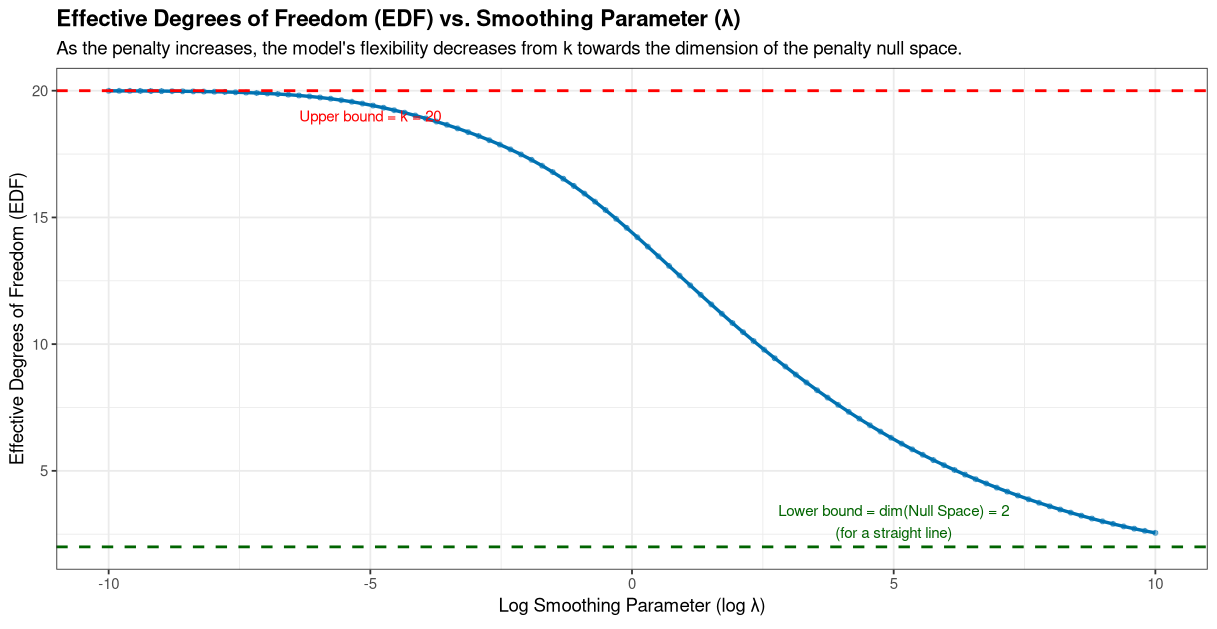
\includegraphics[width=1\linewidth]{edg_viz.png}
 \caption{EDF relationship with increase lambda}
 \label{fig:enter-label-5}
\end{figure}

\newpage
\section{Comparison of Key Spline Bases}
This section provides a detailed comparison of three prominent spline bases: P-splines, Thin Plate Regression Splines, and Adaptive Smoothers.

\begin{figure}[h!]
 \centering
 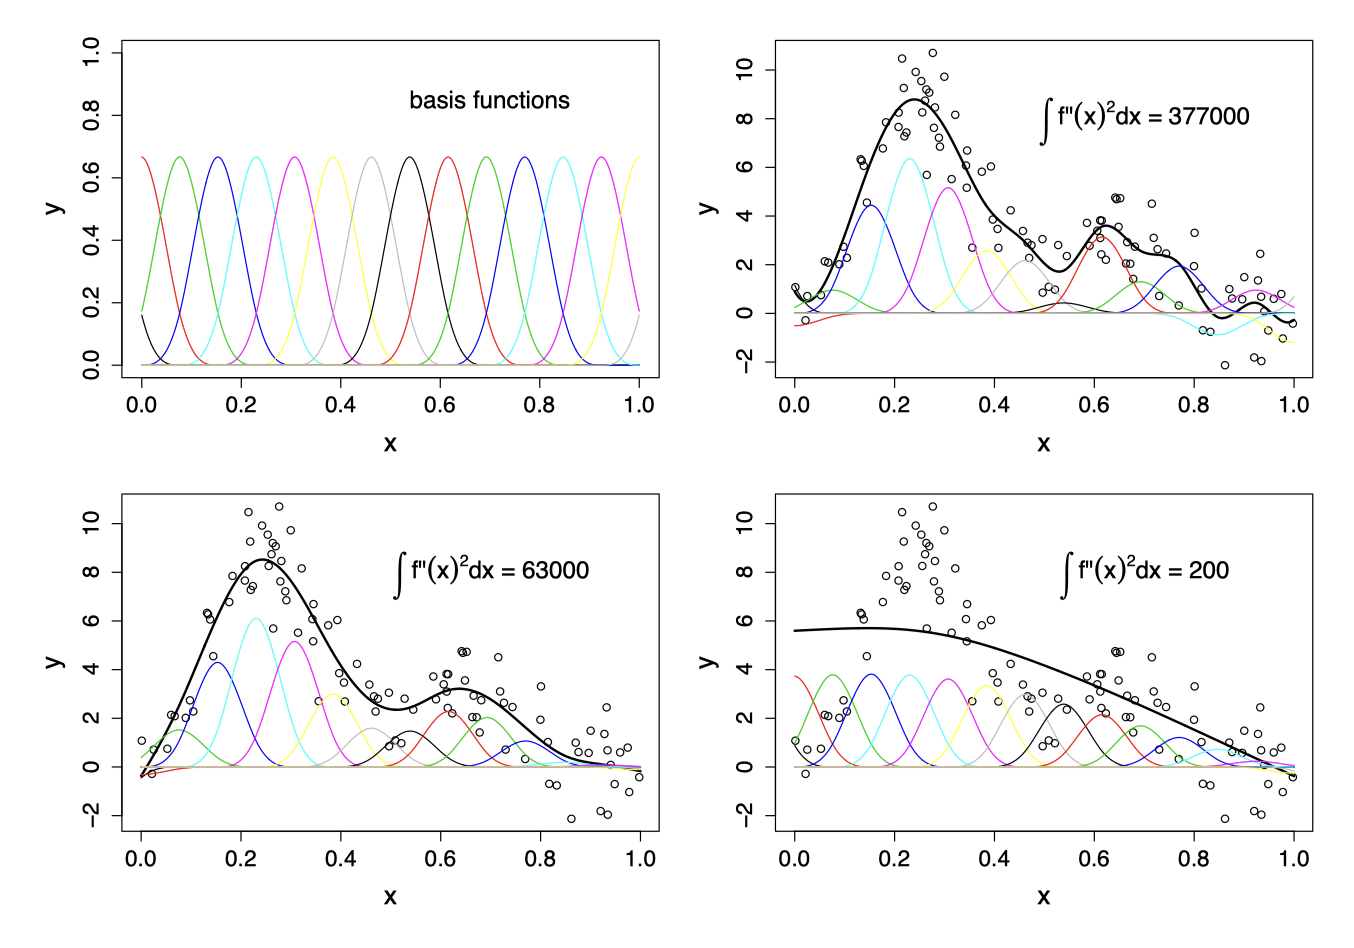
\includegraphics[width=\linewidth]{basis-penalty-illustration.png}
 \caption{Basis Penalty Illustration based on Wood, Basis Penalty Smoothers}
 \label{fig:enter-label-6}
\end{figure}
\subsection{4.1 P-Splines (`bs="ps"`)}
P-splines, introduced by Eilers and Marx (1996), represent a practical and computationally efficient approach to penalized spline smoothing. They combine a B-spline basis with a discrete penalty based on finite differences of adjacent B-spline coefficients.

\paragraph{Basis: B-splines with Evenly Spaced Knots}
P-splines employ B-spline basis functions $b_k(x)$. As detailed in Section 3.1, B-splines are piecewise polynomials of a specified degree (cubic B-splines are a common choice) and possess local support, meaning each $b_k(x)$ is non-zero only over a few adjacent knot intervals.
A defining characteristic of P-splines is the use of a relatively large number of knots that are \textbf{evenly spaced} over the domain of the covariate $x$. This deliberate choice simplifies the construction of the penalty matrix and, more importantly, makes the precise number and location of knots non-critical for the quality of the fit, as the effective smoothness is primarily controlled by the smoothing parameter $\lambda$ associated with the penalty. The number of basis functions, $K$, is typically chosen to be moderately large (e.g., $K=10$ to $K=40$) to ensure sufficient flexibility to capture complex patterns if present. 

\paragraph{Penalty: Discrete Differences of Adjacent Coefficients}
The penalty in P-splines targets the differences between coefficients $\beta_k$ of adjacent B-spline basis functions. This is based on the intuition that a smooth function should have smoothly varying B-spline coefficients.
For an $m$-th order difference penalty, the penalty term is $\lambda \sum_{k} (\Delta^m \beta_k)^2$, where $\Delta^m \beta_k$ is the $m$-th order difference.
\begin{itemize}
 \item $\Delta \beta_k = \beta_k - \beta_{k-1}$ (first-order difference)
 \item $\Delta^2 \beta_k = \beta_k - 2\beta_{k-1} + \beta_{k-2}$ (second-order difference, using appropriate indexing for $\beta_k, \beta_{k-1}, \beta_{k-2}$).[17, 25]
 \item $\Delta^3 \beta_k = \beta_k - 3\beta_{k-1} + 3\beta_{k-2} - \beta_{k-3}$ (third-order difference).
\end{itemize}
The penalty matrix takes the form $\mathbf{S} = \mathbf{D}_m^T \mathbf{D}_m$, where $\mathbf{D}_m$ is the matrix operator that computes the $m$-th order differences.
For example, if $K=5$ coefficients $\boldsymbol{\beta} = [\beta_1, \beta_2, \beta_3, \beta_4, \beta_5]^T$:
\begin{itemize}
 \item The first-order difference matrix $\mathbf{D}_1$ (of size $(K-1) \times K$) would be:
 \[ \mathbf{D}_1 = \begin{pmatrix} -1 & 1 & 0 & 0 & 0 \\ 0 & -1 & 1 & 0 & 0 \\ 0 & 0 & -1 & 1 & 0 \\ 0 & 0 & 0 & -1 & 1 \end{pmatrix} \]
 yielding $\mathbf{D}_1 \boldsymbol{\beta} = [\beta_2-\beta_1, \beta_3-\beta_2, \beta_4-\beta_3, \beta_5-\beta_4]^T$.

 \item The second-order difference matrix $\mathbf{D}_2$ (of size $(K-2) \times K$) would be:
 \[ \mathbf{D}_2 = \begin{pmatrix} 1 & -2 & 1 & 0 & 0 \\ 0 & 1 & -2 & 1 & 0 \\ 0 & 0 & 1 & -2 & 1 \end{pmatrix} \]
 yielding $\mathbf{D}_2 \boldsymbol{\beta} = [\beta_1-2\beta_2+\beta_3, \beta_2-2\beta_3+\beta_4, \beta_3-2\beta_4+\beta_5]^T$. (Note: The exact form of differences, e.g., forward, backward, or centered, can vary, but the principle of penalizing $m$-th order differences remains. The matrix shown corresponds to centered differences for the interior coefficients if we imagine the sequence $\beta_k$).

 \item The third-order difference matrix $\mathbf{D}_3$ (of size $(K-3) \times K$) would be:
 \[ \mathbf{D}_3 = \begin{pmatrix} -1 & 3 & -3 & 1 & 0 \\ 0 & -1 & 3 & -3 & 1 \end{pmatrix} \]
 yielding $\mathbf{D}_3 \boldsymbol{\beta} = [-\beta_1+3\beta_2-3\beta_3+\beta_4, -\beta_2+3\beta_3-3\beta_4+\beta_5]^T$.
\end{itemize}
The matrix $\mathbf{D}_m$ is sparse (banded), and consequently, $\mathbf{S} = \mathbf{D}_m^T \mathbf{D}_m$ is also sparse (banded), which leads to significant computational efficiencies.[34]

\paragraph{Advantages and Characteristics}
P-splines offer several advantages:
\begin{itemize}
 \item \textbf{Computational Simplicity and Efficiency:} The use of B-splines with equally spaced knots and sparse difference penalty matrices makes P-splines easy to construct and computationally efficient, especially for large datasets.[34]
 \item \textbf{Intuitive Penalty:} The difference penalty is conceptually straightforward; it directly penalizes rapid changes in the sequence of B-spline coefficients.
 \item \textbf{Flexibility in Orders:} P-splines allow for flexible "mixing-and-matching" of the B-spline basis order (e.g., linear, quadratic, cubic B-splines) and the order of the difference penalty ($m$).[34] A common choice is cubic B-splines with a second or third-order difference penalty.
 \item \textbf{Good Performance:} They are often a "workhorse" for univariate smoothing in GAMs due to their good empirical performance and robustness.
 \item \textbf{Bayesian Connection:} The P-spline penalty has a direct Bayesian interpretation as imposing a Gaussian random walk prior on the B-spline coefficients. For instance, a second-order difference penalty corresponds to a second-order random walk prior, $ \beta_k | \beta_{k-1}, \beta_{k-2} \sim N(2\beta_{k-1} - \beta_{k-2}, \sigma_\beta^2) $, where $\sigma_\beta^2$ is related to $1/\lambda$. This connection facilitates Bayesian estimation using MCMC methods and the integration of P-splines into hierarchical Bayesian models.
\end{itemize}


\subsection{4.2 Thin Plate Regression Splines (`bs="tp"`): The Eigen-Based Approach}
Thin Plate Splines (TPS) are a class of smoothers that are optimal in the sense that they minimize a "bending energy" functional, generalizing the draftsman's physical spline to multiple dimensions. Full TPS involve a basis function for each data point, making them computationally intensive for large datasets ($O(n^3)$ complexity). Thin Plate \textit{Regression} Splines (TPRS), as developed by Wood (2003), address this by constructing an optimal, lower-rank approximate basis, thereby avoiding explicit knot selection and significantly reducing computational cost.

\paragraph{The Thin Plate Spline Penalty Functional}
The penalty for a thin plate spline measures its "wiggliness" by integrating squared $m$-th order partial derivatives over the domain of the covariates. For a function $f(\mathbf{x})$ of $d$ covariates, the general penalty functional is:
\[ J_{m,d}(f) = \sum_{\nu_1+\dots+\nu_d = m} \frac{m!}{\nu_1! \dots \nu_d!} \int \left( \frac{\partial^m f}{\partial x_1^{\nu_1} \dots \partial x_d^{\nu_d}} \right)^2 d\mathbf{x} \]
A common case is $m=2$. For $d=1$, this reduces to $\int (f''(x))^2 dx$. For $d=2$ (covariates $x_1, x_2$), the $m=2$ penalty is:
\[ J_{2,2}(f) = \iint \left\{ \left(\frac{\partial^2 f}{\partial x_1^2}\right)^2 + 2\left(\frac{\partial^2 f}{\partial x_1 \partial x_2}\right)^2 + \left(\frac{\partial^2 f}{\partial x_2^2}\right)^2 \right\} dx_1 dx_2 \]
This penalty is isotropic, meaning it penalizes curvature equally in all directions, which is appropriate when covariates are on comparable scales or when no specific directional preference for smoothness exists.

\paragraph{The Null Space of the Penalty}
The TPS penalty $J_{m,d}(f)$ is zero for any polynomial in $d$ variables of total degree less than $m$. These functions form the \textbf{null space} of the penalty and are not penalized by $\mathbf{S}$. For example, if $m=2$, the null space consists of linear functions (and constants), and its dimension is $M = \binom{m+d-1}{d} = \binom{d+1}{d} = d+1$. These $M$ polynomial basis functions must be included in the spline basis and are estimated without shrinkage by the penalty term.

\paragraph{Eigen-Decomposition and Optimal Basis Construction}
The core idea of TPRS is to find a low-rank basis that best approximates the full thin plate spline. This is achieved through an eigen-decomposition related to the penalty structure 
\begin{enumerate}
 \item \textbf{Full Penalty and Basis:} Conceptually, one starts with a basis and penalty structure corresponding to a full TPS (e.g., knots at all unique data locations). Let $\mathbf{S}_{full}$ be the penalty matrix associated with this full basis.
 \item \textbf{Eigen-decomposition:} The penalty matrix $\mathbf{S}_{full}$ (or a related matrix derived from it in the construction of TPRS, see Wood (2003) ) undergoes an eigen-decomposition: $\mathbf{S}_{full} = \mathbf{U \Lambda U}^T$. The columns of $\mathbf{U}$ are the eigenvectors, and $\mathbf{\Lambda}$ is a diagonal matrix of corresponding eigenvalues.
 \item \textbf{Identifying Unpenalized and Penalized Components:}
 \begin{itemize}
\item The $M$ eigenvectors corresponding to zero eigenvalues of $\mathbf{S}_{full}$ span the null space of the penalty (the unpenalized polynomials).
\item The eigenvectors corresponding to positive eigenvalues span the space of "wiggly" functions that are subject to penalization. The magnitude of an eigenvalue $\Lambda_{ii}$ reflects the degree of wiggliness associated with its corresponding eigenvector $\mathbf{u}_i$: smaller positive eigenvalues correspond to smoother functions (less penalty per unit norm of coefficients), while larger eigenvalues correspond to more wiggly functions.
 \end{itemize}
 \item \textbf{Optimal Truncation for Rank-$k$ Basis:} To construct a TPRS basis of a specified rank $k$ (where $k$ is typically much smaller than $n$):
\begin{itemize}
\item The $M$ basis functions spanning the null space are always included.
\item From the remaining eigenvectors (those with positive eigenvalues), the $k-M$ eigenvectors corresponding to the $k-M$ \textit{smallest positive} eigenvalues are selected. These represent the "smoothest" functions in the penalized space.[41, 45]
 \end{itemize}
 \item \textbf{Model and Penalty Matrices:} The model matrix $\mathbf{X}$ for the TPRS is formed using these $k$ selected basis functions ( $M$ null space functions and $k-M$ selected eigenvectors). The penalty matrix $\mathbf{S}$ for this TPRS basis becomes diagonal in this reparameterized representation, with entries corresponding to the $k-M$ selected positive eigenvalues and zeros for the $M$ null space components.
\end{enumerate}
This construction ensures that, for a given rank $k$, the TPRS basis is the best $k$-dimensional approximation to the full TPS in terms of minimizing the perturbation to the smoothing problem.[37]

\paragraph{Reparameterization and Simplified Penalty}
If the original spline coefficients are $\boldsymbol{\beta}$ and the coefficients for the eigenbasis are $\boldsymbol{\alpha}$ (such that $\boldsymbol{\beta} = \mathbf{U}\boldsymbol{\alpha}$), the penalty term $\lambda \boldsymbol{\beta}^T \mathbf{S}_{full} \boldsymbol{\beta}$ transforms to $\lambda \boldsymbol{\alpha}^T \mathbf{\Lambda} \boldsymbol{\alpha} = \lambda \sum_{i=1}^{K} \Lambda_{ii} \alpha_i^2$. The truncation step effectively sets $\alpha_i = 0$ for the components corresponding to the discarded eigenvectors (those with large eigenvalues, representing very wiggly functions). For the selected $k-M$ penalized components, the penalty is $\lambda \sum_{j=1}^{k-M} \Lambda_{j}^* \alpha_j^{*2}$, where $\Lambda_j^*$ are the smallest positive eigenvalues.

\paragraph{Advantages and Characteristics}
\begin{itemize}
 \item \textbf{Knot-free Definition:} TPRS entirely avoids the subjective and often problematic process of knot selection. The basis dimension $k$ is specified, but not knot locations.
 \item \textbf{Optimality:} The low-rank basis is chosen in a principled way to be an optimal approximation of the full thin plate spline, minimizing information loss for a given basis size.[37]
 \item \textbf{Multi-dimensional Smoothing:} TPRS are naturally defined for any number of covariates $d$ and are particularly well-suited for modeling interactions and smooth surfaces in multiple dimensions.
 \item \textbf{Isotropy:} The standard TPRS penalty is isotropic, treating all covariates (and directions in the covariate space) equally in terms of smoothing. This is an advantage when covariates are on similar scales and no prior knowledge suggests directional differences in smoothness.
\end{itemize}
The eigen-decomposition approach of TPRS is conceptually related to Principal Components Analysis (PCA). Just as PCA identifies principal components that capture the most variance, the eigen-decomposition here identifies basis functions (eigenfunctions of the penalty operator) that are ordered by their intrinsic smoothness (or wiggliness, as quantified by the eigenvalues). By selecting the smoothest of these, TPRS constructs a reduced-rank basis that retains the most important smooth features. TPRS are a default choice for multi-dimensional smoothing in `mgcv` due to these desirable properties.[38]

\subsection{4.3 Adaptive Smoothers (`bs="ad"`)}
Standard penalized splines assume that the optimal degree of smoothness is constant across the entire domain of the covariate(s). However, many real-world functions exhibit varying complexity: they might be very smooth (nearly linear) in some regions and highly variable or oscillatory in others. An adaptive smoother is designed for such situations by allowing the penalty strength, and thus the effective smoothness of the fit, to vary with the covariate values.

\paragraph{Intuition: The Smart Sander Analogy}
Imagine sanding a piece of wood that has some very rough patches and some nearly finished patches. Using a standard smoother (like a P-spline with a single $\lambda$) is analogous to using the same grit sandpaper across the entire piece. It might work reasonably well if the wood is uniformly rough, but it's a compromise. You would risk either oversanding the smooth parts (losing detail) or undersanding the rough parts (leaving them unfinished). An adaptive smoother is like a "smart sander" that automatically senses the local roughness of the wood and adjusts its grit size accordingly—using coarse grit on the rough patches and fine grit on the smooth ones.

\paragraph{Mechanism: Spatially Varying Penalty Weights}
The adaptive smoother in `mgcv` (`bs="ad"`) achieves this by modifying the standard P-spline penalty. A regular P-spline penalty is $\mathcal{P} = \lambda \sum_{k} (\Delta^m \beta_k)^2$. The adaptive version introduces spatially-varying weights, $\omega_k$:
\[ \mathcal{P}_a = \lambda \sum_{k} \omega_k (\Delta^m \beta_k)^2 \]
These weights $\omega_k > 0$ control the local penalty strength:
\begin{itemize}
 \item Where $\omega_k$ is \textbf{large}, the penalty is strong, forcing the function to be locally smooth.
 \item Where $\omega_k$ is \textbf{small}, the penalty is weak, allowing the function to be locally wiggly to capture rapid changes in the data.
\end{itemize}
In matrix form, the penalty is $\lambda \boldsymbol{\beta}^T \mathbf{D}_m^T \text{diag}(\boldsymbol{\omega}) \mathbf{D}_m \boldsymbol{\beta}$.

covariate, $x$, say. For example consider a second order P-spline penalty in which the squared differences are now weighted
$$
P_a = \sum_{i=2}^{k-1} \omega_i(\beta_{i-1} - 2\beta_i + \beta_{i+1})^2 = \boldsymbol{\beta}^\mathrm{T} \mathbf{D}^\mathrm{T} \mathrm{diag}(\boldsymbol{\omega}) \mathbf{D} \boldsymbol{\beta}
$$
$$
\text{where } \mathbf{D} = \begin{bmatrix}
1 & -2 & 1 & 0 & \cdot \\
0 & 1 & -2 & 1 & \cdot \\
\cdot & \cdot & \cdot & \cdot & \cdot \\
\cdot & \cdot & \cdot & \cdot & \cdot
\end{bmatrix}.
$$
Now let the weights $\omega_i$ vary smoothly with $i$ and hence with $x$. An obvious way to do this is to use a B-spline basis expansion $\boldsymbol{\omega} = \mathbf{B\lambda}$, where $\boldsymbol{\lambda}$ is the vector of basis coefficients. Then, writing $\mathbf{B}_{.j}$ for the $j^\text{th}$ column of $\mathbf{B}$ we have
$$
\boldsymbol{\beta}^\mathrm{T} \mathbf{D}^\mathrm{T} \mathrm{diag}(\boldsymbol{\omega}) \mathbf{D} \boldsymbol{\beta} = \sum_j \lambda_j \boldsymbol{\beta}^\mathrm{T} \mathbf{D}^\mathrm{T} \mathrm{diag}(\mathbf{B}_{.j}) \mathbf{D} \boldsymbol{\beta} = \sum_j \lambda_j \boldsymbol{\beta}^\mathrm{T} \mathbf{S}_j \boldsymbol{\beta}.
$$

\paragraph{How are the Weights Determined?}
The key innovation is that the weights $\omega_k$ are not pre-specified but are themselves estimated from the data. They are modeled as a smooth function of their index $k$ (which corresponds to location along the covariate $x$). To ensure the weights vary smoothly and remain positive, their logarithm is typically modeled using another spline (a "meta-spline"):
\[ \log(\omega_k) = \sum_{j=1}^{K_{\omega}} \gamma_j b_{\omega,j}(k) \quad \text{or in matrix form} \quad \log(\boldsymbol{\omega}) = \mathbf{B}_{\omega}\boldsymbol{\gamma} \]
Here, $\mathbf{B}_{\omega}$ is a basis matrix (e.g., a B-spline basis) for the log-weights, and $\boldsymbol{\gamma}$ are the coefficients of this meta-spline. These coefficients $\boldsymbol{\gamma}$ effectively become additional smoothing parameters for the model. The model now has multiple smoothing parameters to estimate, which control how the main penalty varies.

The model is fitted using an iterative process that alternates between estimating the main function and estimating the penalty weights. This allows the smoother to "learn" where it needs to be more or less flexible. This hierarchical structure—a spline for the function whose penalty is controlled by another spline—is why it can be thought of as a GAM within a GAM penalty.

While powerful, adaptive smoothers are more complex and have more parameters to estimate. They generally require more data than standard smoothers to reliably estimate the varying smoothness structure and are computationally more intensive. They are particularly useful when visual inspection of the data or prior knowledge suggests that the assumption of constant smoothness is likely to be violated.
\begin{figure}[h!]
 \centering
 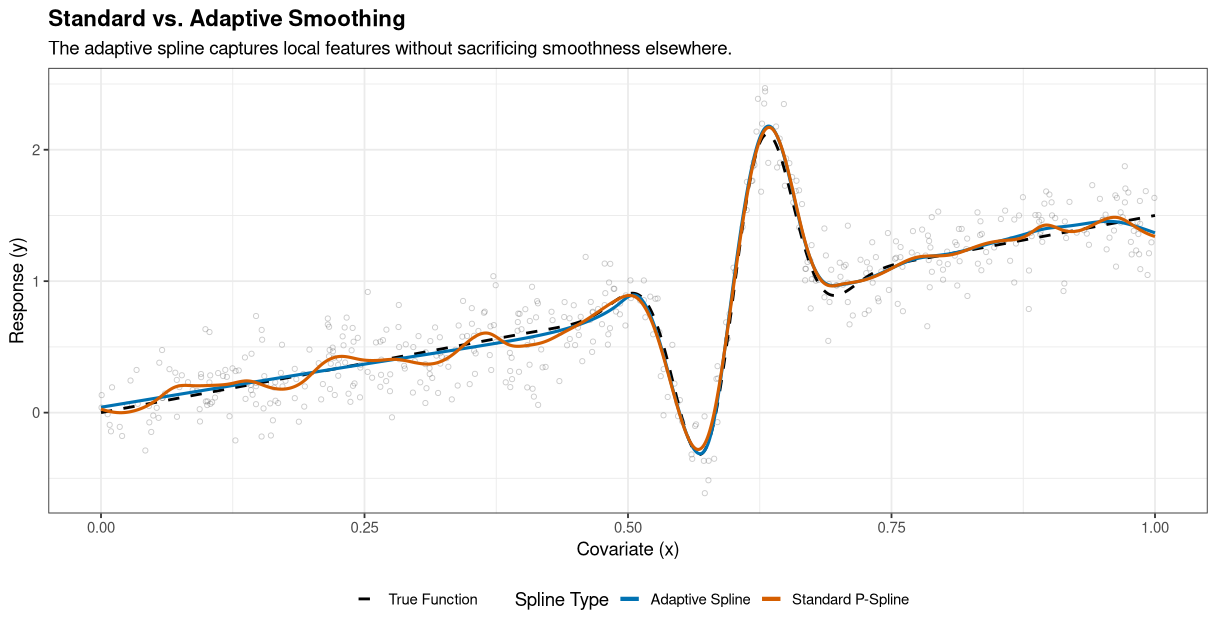
\includegraphics[width=1\linewidth]{adaptive_spline.png}
 \caption{Adaptive vs P-Spline}
\end{figure}

\vspace{1em}
\begin{table}[h!]
\centering
\caption{Comparison of Key Penalized Spline Bases in `mgcv`}
\label{tab:spline_comparison}
\begin{tabular}{@{}lllll@{}}
\toprule
\textbf{\texttt{mgcv} ID} & \textbf{Spline Type Name} & \textbf{Underlying Basis} & \textbf{Knot Strategy} & \textbf{Penalty Nature} \\
\midrule
`bs="ps"` & P-Spline & B-splines & Evenly spaced (many) & Discrete differences \\
& & (e.g., cubic) & User specifies $K$ & of coefficients \\
& & & & (e.g., $\sum (\Delta^2 \beta_k)^2$) \\
\addlinespace
`bs="tp"` & Thin Plate & Eigenfunctions of & Knot-free (implicit); & Integrated squared \\
& Regression Spline & TPS operator & User specifies basis rank $k$ & $m$-th derivatives \\
& & & &  \\
\addlinespace
`bs="ad"` & Adaptive P-Spline & B-splines for function; & Evenly spaced for & Weighted discrete \\
& & B-splines for penalty & underlying P-spline & differences of coeff. \\
& & weights & & $\sum \omega_k (\Delta^m \beta_k)^2$ \\
\bottomrule
\end{tabular}
\par
\vspace{0.5em}
\textit{Note:} $K$ is the number of basis functions. $\Delta^m \beta_k$ is the $m$-th order difference of coefficients. $\omega_k$ are spatially varying weights.
\end{table}

\newpage
\section{Penalized Likelihood and Bayesian Inference}
The framework of penalized splines possesses deep connections to Bayesian statistical methodology. This section establishes the mathematical equivalence between penalized likelihood estimation and Bayesian inference, derives the posterior distribution of the spline coefficients, and explores different approaches for handling the smoothing parameter—from frequentist tuning to full Bayesian hierarchical modeling.

\subsection{5.1 The Core Connection: From Penalized Likelihood to Bayesian Posterior}
The penalized least squares objective function used in spline estimation has a profound interpretation: it is mathematically equivalent to the negative log-posterior density of a specific Bayesian model. This section establishes this equivalence and derives the resulting posterior distribution.

\paragraph{The Penalized Likelihood Framework}
Recall that penalized spline estimation seeks to minimize:
\[ \mathcal{L}_{pen}(\boldsymbol{\beta}) = ||\mathbf{y} - \mathbf{X}\boldsymbol{\beta}||^2 + \lambda \boldsymbol{\beta}^T \mathbf{S} \boldsymbol{\beta} \]
where $\mathbf{y}$ is the response vector, $\mathbf{X}$ is the design matrix containing the spline basis functions, $\boldsymbol{\beta}$ are the coefficients to be estimated, $\lambda$ is the smoothing parameter, and $\mathbf{S}$ is the penalty matrix encoding the roughness of the function.

\paragraph{The Bayesian Interpretation}
To establish the Bayesian connection, we specify a probabilistic model with the following components:

\begin{enumerate}
\item \textbf{Likelihood}: Assume the data arise from a Gaussian model with errors $\epsilon_i \sim N(0, \sigma^2)$:
\[ \mathbf{y} | \boldsymbol{\beta}, \sigma^2 \sim N(\mathbf{X}\boldsymbol{\beta}, \sigma^2\mathbf{I}) \]
This gives the likelihood:
\[ P(\mathbf{y} | \boldsymbol{\beta}, \sigma^2) = (2\pi\sigma^2)^{-n/2} \exp\left(-\frac{1}{2\sigma^2}||\mathbf{y} - \mathbf{X}\boldsymbol{\beta}||^2\right) \]

\item \textbf{Prior}: Specify a Gaussian prior on the coefficients that encodes smoothness:
\[ \boldsymbol{\beta} | \lambda, \sigma^2 \sim N(\mathbf{0}, \sigma^2\lambda^{-1}\mathbf{S}^{-}) \]
where $\mathbf{S}^{-}$ is a generalized inverse of the penalty matrix. This prior has the form:
\[ P(\boldsymbol{\beta} | \lambda, \sigma^2) \propto \exp\left(-\frac{\lambda}{2\sigma^2}\boldsymbol{\beta}^T\mathbf{S}\boldsymbol{\beta}\right) \]
\end{enumerate}

The prior encodes the belief that smoother functions (those with smaller $\boldsymbol{\beta}^T\mathbf{S}\boldsymbol{\beta}$) are more probable. The parameter $\lambda/\sigma^2$ controls the strength of this smoothness preference.

\paragraph{Equivalence to MAP Estimation}
By Bayes' theorem, the posterior distribution is:
\[ P(\boldsymbol{\beta} | \mathbf{y}, \lambda, \sigma^2) \propto P(\mathbf{y} | \boldsymbol{\beta}, \sigma^2) P(\boldsymbol{\beta} | \lambda, \sigma^2) \]

Taking logarithms:
\begin{align}
\log P(\boldsymbol{\beta} | \mathbf{y}, \lambda, \sigma^2) &\propto -\frac{1}{2\sigma^2}||\mathbf{y} - \mathbf{X}\boldsymbol{\beta}||^2 - \frac{\lambda}{2\sigma^2}\boldsymbol{\beta}^T\mathbf{S}\boldsymbol{\beta} \\
&= -\frac{1}{2\sigma^2}\left(||\mathbf{y} - \mathbf{X}\boldsymbol{\beta}||^2 + \lambda\boldsymbol{\beta}^T\mathbf{S}\boldsymbol{\beta}\right)
\end{align}

Maximizing this log-posterior with respect to $\boldsymbol{\beta}$ is equivalent to minimizing:
\[ ||\mathbf{y} - \mathbf{X}\boldsymbol{\beta}||^2 + \lambda\boldsymbol{\beta}^T\mathbf{S}\boldsymbol{\beta} \]

This is precisely the penalized least squares objective function. Therefore, the penalized least squares estimate $\hat{\boldsymbol{\beta}}$ is the Maximum A Posteriori (MAP) estimate under this Bayesian model.

\subsection{5.2 The Key Result: Posterior Distribution of $\boldsymbol{\beta}$}
While the MAP estimate provides a point estimate, the full Bayesian framework yields the complete posterior distribution of the coefficients. This result is fundamental for uncertainty quantification and forms the basis for constructing Bayesian confidence bands.

\paragraph{Derivation of the Posterior Distribution}
Given the Gaussian likelihood and Gaussian prior, the posterior distribution of $\boldsymbol{\beta}$ is also Gaussian. To derive its form, we complete the square in the log-posterior:

\begin{align}
\log P(\boldsymbol{\beta} | \mathbf{y}, \lambda, \sigma^2) &\propto -\frac{1}{2\sigma^2}\left[||\mathbf{y} - \mathbf{X}\boldsymbol{\beta}||^2 + \lambda\boldsymbol{\beta}^T\mathbf{S}\boldsymbol{\beta}\right] \\
&= -\frac{1}{2\sigma^2}\left[(\mathbf{y} - \mathbf{X}\boldsymbol{\beta})^T(\mathbf{y} - \mathbf{X}\boldsymbol{\beta}) + \lambda\boldsymbol{\beta}^T\mathbf{S}\boldsymbol{\beta}\right] \\
&= -\frac{1}{2\sigma^2}\left[\mathbf{y}^T\mathbf{y} - 2\mathbf{y}^T\mathbf{X}\boldsymbol{\beta} + \boldsymbol{\beta}^T\mathbf{X}^T\mathbf{X}\boldsymbol{\beta} + \lambda\boldsymbol{\beta}^T\mathbf{S}\boldsymbol{\beta}\right] \\
&= -\frac{1}{2\sigma^2}\left[\boldsymbol{\beta}^T(\mathbf{X}^T\mathbf{X} + \lambda\mathbf{S})\boldsymbol{\beta} - 2\mathbf{y}^T\mathbf{X}\boldsymbol{\beta} + \mathbf{y}^T\mathbf{y}\right]
\end{align}

Completing the square in $\boldsymbol{\beta}$:
\begin{align}
&= -\frac{1}{2\sigma^2}\left[(\boldsymbol{\beta} - \hat{\boldsymbol{\beta}})^T(\mathbf{X}^T\mathbf{X} + \lambda\mathbf{S})(\boldsymbol{\beta} - \hat{\boldsymbol{\beta}}) + \text{const}\right]
\end{align}
where $\hat{\boldsymbol{\beta}} = (\mathbf{X}^T\mathbf{X} + \lambda\mathbf{S})^{-1}\mathbf{X}^T\mathbf{y}$.

\paragraph{The Posterior Distribution}
This shows that the posterior distribution is:
\[ \boxed{\boldsymbol{\beta} | \mathbf{y}, \lambda, \sigma^2 \sim N(\hat{\boldsymbol{\beta}}, \mathbf{V}_{\beta})} \]
where:
\begin{itemize}
\item $\hat{\boldsymbol{\beta}} = (\mathbf{X}^T\mathbf{X} + \lambda\mathbf{S})^{-1}\mathbf{X}^T\mathbf{y}$ is the posterior mean (and the penalized least squares estimate)
\item $\mathbf{V}_{\beta} = \sigma^2(\mathbf{X}^T\mathbf{X} + \lambda\mathbf{S})^{-1}$ is the posterior covariance matrix
\end{itemize}

\paragraph{Implications for Inference}
This result has several important implications:

\begin{enumerate}
\item \textbf{Point Estimation}: The penalized least squares estimate $\hat{\boldsymbol{\beta}}$ is not just the MAP estimate but also the posterior mean and median (due to symmetry of the Gaussian).

\item \textbf{Uncertainty Quantification}: The posterior covariance matrix $\mathbf{V}_{\beta}$ provides full uncertainty quantification for the coefficients. The diagonal elements give the posterior variances of individual coefficients.

\item \textbf{Bayesian Confidence Bands}: For the fitted function at a point $\mathbf{x}_0$, we have:
\[ f(\mathbf{x}_0) | \mathbf{y}, \lambda, \sigma^2 \sim N(\mathbf{x}_0^T\hat{\boldsymbol{\beta}}, \mathbf{x}_0^T\mathbf{V}_{\beta}\mathbf{x}_0) \]
This allows construction of pointwise Bayesian confidence bands for the smooth function.

\item \textbf{Comparison to Unpenalized Regression}: In the limit $\lambda \to 0$, we recover $\mathbf{V}_{\beta} \to \sigma^2(\mathbf{X}^T\mathbf{X})^{-1}$, the standard OLS covariance matrix.
\end{enumerate}

\paragraph{The Role of the Smoothing Parameter}
Note that the posterior distribution depends on both $\lambda$ and $\sigma^2$. In the results above, these are treated as known. The remainder of this section addresses different approaches for handling these parameters: treating them as fixed (frequentist), estimating them via marginal likelihood (Empirical Bayes), or placing priors on them (Full Bayes).

\subsection{5.3 Methods for Selecting the Smoothing Parameter}
The smoothing parameter $\lambda$ plays a crucial role in determining the balance between fit and smoothness. This section presents three major approaches for its selection, progressing from frequentist to fully Bayesian methods.

\subsubsection{5.3.1 Generalized Cross-Validation (GCV): The Frequentist Approach}
From a frequentist perspective, $\lambda$ is a tuning parameter to be selected by optimizing a criterion that estimates out-of-sample prediction error.

\paragraph{Leave-One-Out Cross-Validation}
The ideal approach would be Leave-One-Out Cross-Validation (LOOCV), where for each observation $i$:
\begin{enumerate}
\item Fit the model using all data except $(x_i, y_i)$, obtaining $\hat{f}_{(-i)}$
\item Predict $y_i$ using $\hat{f}_{(-i)}(x_i)$
\item Compute the squared prediction error $(y_i - \hat{f}_{(-i)}(x_i))^2$
\end{enumerate}
The LOOCV score is: $CV(\lambda) = \frac{1}{n} \sum_{i=1}^n (y_i - \hat{f}_{(-i)}(x_i))^2$

\paragraph{The GCV Approximation}
For linear smoothers where $\hat{\mathbf{y}} = \mathbf{A}(\lambda)\mathbf{y}$ with influence matrix:
\[ \mathbf{A}(\lambda) = \mathbf{X}(\mathbf{X}^T\mathbf{X} + \lambda\mathbf{S})^{-1}\mathbf{X}^T \]

A remarkable result shows that:
\[ CV(\lambda) = \frac{1}{n} \sum_{i=1}^n \left( \frac{y_i - \hat{y}_i(\lambda)}{1 - A_{ii}(\lambda)} \right)^2 \]
where $A_{ii}(\lambda)$ is the $i$-th diagonal element of $\mathbf{A}(\lambda)$.

GCV approximates this by replacing individual leverages $A_{ii}(\lambda)$ with their average:
\[ \mathcal{V}_g(\lambda) = \frac{n \cdot \text{RSS}(\lambda)}{[n - \text{tr}(\mathbf{A}(\lambda))]^2} \]
where:
\begin{itemize}
\item $\text{RSS}(\lambda) = ||\mathbf{y} - \mathbf{A}(\lambda)\mathbf{y}||^2$ is the residual sum of squares
\item $\text{tr}(\mathbf{A}(\lambda))$ is the effective degrees of freedom (EDF)
\end{itemize}

The optimal $\lambda$ minimizes $\mathcal{V}_g(\lambda)$. While computationally efficient, GCV can undersmooth (select too small $\lambda$) in small samples.

\subsubsection{5.3.2 REML: The Empirical Bayes Approach}
The Bayesian interpretation naturally suggests selecting $\lambda$ by maximizing the marginal likelihood—the probability of the data after integrating out the coefficients.

\paragraph{The Marginal Likelihood}
The marginal likelihood is obtained by integrating over all possible values of $\boldsymbol{\beta}$:
\[ P(\mathbf{y}|\lambda, \sigma^2) = \int P(\mathbf{y}|\boldsymbol{\beta}, \sigma^2) P(\boldsymbol{\beta}|\lambda, \sigma^2) d\boldsymbol{\beta} \]

For our Gaussian model, this integral has a closed form. Using properties of multivariate Gaussians:
\[ \mathbf{y}|\lambda, \sigma^2 \sim N(\mathbf{0}, \mathbf{C}_y) \]
where $\mathbf{C}_y = \sigma^2(\mathbf{I} + \lambda^{-1}\mathbf{X}\mathbf{S}^{-}\mathbf{X}^T)$.

\paragraph{Connection to Mixed Models}
A key insight is that penalized splines can be reformulated as linear mixed models:
\begin{itemize}
\item Treat $\boldsymbol{\beta}$ as random effects with distribution $\boldsymbol{\beta} \sim N(\mathbf{0}, \sigma^2_{\beta}\mathbf{S}^{-})$
\item The smoothing parameter becomes a variance ratio: $\lambda = \sigma^2/\sigma^2_{\beta}$
\end{itemize}

\paragraph{Why REML Instead of ML?}
Maximum Likelihood (ML) estimation of variance components is known to be biased in the presence of fixed effects. REML (Restricted Maximum Likelihood) corrects this by:
\begin{enumerate}
\item Working with contrasts of the data that are independent of fixed effects
\item Effectively integrating out the fixed effects before estimating variances
\item Providing unbiased estimates analogous to dividing by $n-p$ instead of $n$
\end{enumerate}

REML estimation of $\lambda$ is generally more stable than GCV, particularly for complex models with multiple smooth terms.

\subsubsection{5.3.3 Full Bayesian Approach: Hyperpriors on $\lambda$}
The fully Bayesian approach treats $\lambda$ (and $\sigma^2$) as random variables with their own prior distributions.

\paragraph{Hierarchical Model Specification}
The complete hierarchical model becomes:
\begin{align}
\text{Data Level:} \quad & \mathbf{y} | \boldsymbol{\beta}, \sigma^2 \sim N(\mathbf{X}\boldsymbol{\beta}, \sigma^2\mathbf{I}) \\
\text{Process Level:} \quad & \boldsymbol{\beta} | \lambda, \sigma^2 \sim N(\mathbf{0}, \sigma^2\lambda^{-1}\mathbf{S}^{-}) \\
\text{Hyperparameter Level:} \quad & \lambda \sim \pi(\lambda), \quad \sigma^2 \sim \pi(\sigma^2)
\end{align}

Common choices for hyperpriors include:
\begin{itemize}
\item For $\sigma^2_{\beta} = \sigma^2/\lambda$: Half-Cauchy or half-Student-t distributions
\item For $\sigma^2$: Inverse-Gamma or half-Student-t on $\sigma$
\end{itemize}

\paragraph{Posterior Inference via MCMC}
The joint posterior $P(\boldsymbol{\beta}, \lambda, \sigma^2 | \mathbf{y})$ is typically intractable. Markov Chain Monte Carlo (MCMC) methods are used to sample from this distribution:
\begin{itemize}
\item Gibbs sampling for conjugate components
\item Hamiltonian Monte Carlo (HMC) for efficient exploration
\item No-U-Turn Sampler (NUTS) as implemented in Stan
\end{itemize}

\paragraph{Advantages of the Full Bayesian Approach}
\begin{enumerate}
\item \textbf{Complete Uncertainty Quantification}: Uncertainty in $\lambda$ and $\sigma^2$ is propagated to all inferences
\item \textbf{Automatic Multiplicity Adjustment}: Multiple testing issues are naturally handled
\item \textbf{Hyperprior Regularization}: Hyperpriors can stabilize estimation in difficult cases
\item \textbf{Model Averaging}: Can average over different values of $\lambda$ weighted by posterior probability
\end{enumerate}

The main disadvantage is computational cost, though modern MCMC algorithms have made this increasingly tractable.

\subsection{5.4 Practical Implications and Software Implementation}

\paragraph{Uncertainty Quantification Under Different Approaches}
The treatment of $\lambda$ has important implications for uncertainty quantification:

\begin{enumerate}
\item \textbf{Conditional on $\hat{\lambda}$ (GCV/REML)}: Uses $\mathbf{V}_{\beta} = \sigma^2(\mathbf{X}^T\mathbf{X} + \hat{\lambda}\mathbf{S})^{-1}$
   \begin{itemize}
   \item Treats $\hat{\lambda}$ as fixed in subsequent inference
   \item May underestimate uncertainty, especially in small samples
   \item Computationally efficient
   \end{itemize}

\item \textbf{Accounting for $\lambda$ Uncertainty (Full Bayes)}: 
   \begin{itemize}
   \item Posterior variance includes additional component from $\lambda$ uncertainty
   \item More honest uncertainty quantification
   \item Wider confidence/credible intervals
   \end{itemize}
\end{enumerate}

\paragraph{Software Implementation}
Modern implementations handle these approaches efficiently:
\begin{itemize}
\item \texttt{mgcv} in R: Default uses REML, options for GCV and other criteria
\item \texttt{brms}/\texttt{rstanarm}: Full Bayesian implementation via Stan
\item \texttt{BayesX}: Specialized software for Bayesian GAMs
\item \texttt{INLA}: Approximate Bayesian inference avoiding MCMC
\end{itemize}

\paragraph{Recommendations for Practice}
\begin{enumerate}
\item For exploratory analysis: GCV provides quick results
\item For final models: REML offers better stability
\item For critical applications: Full Bayes provides most complete inference
\item For large datasets: Empirical Bayes (REML) balances accuracy and speed
\item For small datasets or complex models: Full Bayes may be necessary
\end{enumerate}

\subsection{5.5 Summary}
This section has established the deep connection between penalized spline estimation and Bayesian inference. The key insights are:

\begin{enumerate}
\item The penalized least squares estimate is the posterior mean under a specific Bayesian model
\item The posterior distribution $\boldsymbol{\beta}|\mathbf{y} \sim N(\hat{\boldsymbol{\beta}}, \mathbf{V}_{\beta})$ provides complete inference
\item Different approaches to handling $\lambda$ represent different levels of Bayesian modeling:
   \begin{itemize}
   \item GCV: Frequentist cross-validation
   \item REML: Empirical Bayes via marginal likelihood
   \item Full Bayes: Complete hierarchical modeling
   \end{itemize}
\item The choice of approach involves trade-offs between computational cost, statistical efficiency, and completeness of inference
\end{enumerate}

This Bayesian perspective not only provides theoretical insight but also practical tools for uncertainty quantification, model selection, and robust inference in the presence of smoothing parameters.
\section{The Spline-Random Effect Duality}
 This section explicitly details the mathematical connection between penalized splines and random effects within a mixed effects model framework., showing how a standard random effect is just a special type of penalized smoother and how, conversely, any penalized smoother can be represented as a random effect.

\subsection{7.1 How Random Effects are Fitted as Splines (`bs="re"`)}
In mgcv, a standard random intercept term, such as one might fit for different groups or, in your case, `Village`, is specified using the `s()` function with the basis argument `bs="re"`. For a factor variable `z` with $J$ levels, a term like `s(z, bs="re")` is included in the model formula.

\paragraph{The "Basis" and Penalty for a Random Effect}
How is this a spline? The trick is to define a "basis" and a penalty that recovers the familiar random effects structure.
\begin{enumerate}
    \item \textbf{The Model Matrix $\mathbf{X}$:} For each of the $J$ levels of the factor `z`, a simple indicator variable is created. If the model is `y ~ s(z, bs="re")`, the model matrix $\mathbf{X}$ for this term is an $n \times J$ matrix where each row has a `1` in the column corresponding to the level of `z` for that observation, and `0`s elsewhere. The coefficients $\boldsymbol{\beta} = [\beta_1, \dots, \beta_J]^T$ are the random intercepts for each level. The functional form is simply $f(z_i) = \beta_j$ if observation $i$ belongs to group $j$.

    \item \textbf{The Penalty Matrix $\mathbf{S}$:} The key assumption of a standard random intercept model is that the intercepts $\beta_j$ are independent and identically distributed (i.i.d.) random variables, typically from a Gaussian distribution, $\beta_j \sim N(0, \sigma_b^2)$. The goal is to shrink these coefficients towards their overall mean (zero, after centering). This is achieved with a simple \textbf{ridge penalty} or \textbf{identity penalty}. The penalty matrix $\mathbf{S}$ is simply the $J \times J$ identity matrix, $\mathbf{S} = \mathbf{I}$.
\end{enumerate}
The penalty term for a random effect is therefore:
\[ \lambda \boldsymbol{\beta}^T \mathbf{S} \boldsymbol{\beta} = \lambda \boldsymbol{\beta}^T \mathbf{I} \boldsymbol{\beta} = \lambda \sum_{j=1}^{J} \beta_j^2 \]
This penalty directly penalizes the size of the coefficients, shrinking them towards zero. The amount of shrinkage is controlled by $\lambda$.

\paragraph{Connection to LMMs}
In a standard Linear Mixed Model (LMM), the random intercepts are assumed to follow $\beta_j \sim N(0, \sigma_b^2)$, and the errors follow $\epsilon_i \sim N(0, \sigma_e^2)$. The smoothing parameter $\lambda$ in the GAM formulation is directly related to these variance components:
\[ \lambda = \frac{\sigma_e^2}{\sigma_b^2} \]
Estimating $\lambda$ via REML is therefore exactly equivalent to estimating the variance components $\sigma_b^2$ and $\sigma_e^2$ in an LMM. A large random effect variance $\sigma_b^2$ corresponds to a small $\lambda$, imposing little shrinkage. A small $\sigma_b^2$ corresponds to a large $\lambda$, shrinking the random intercepts strongly towards zero.

So, when you fit a term like `s(Village, bs="re")`, `mgcv` is simply setting up a penalized regression with an identity penalty matrix, and the REML/ML machinery estimates the optimal $\lambda$, which is equivalent to estimating the variance of the `Village` random effect.

\subsection{7.2. Why All Penalized Splines are Random Effects}
The previous section showed how a random effect can be written as a special penalized term. Now we show the general case: any penalized term in a GAM can be formally expressed as a random effect in a mixed model. This provides the theoretical justification for using LMM estimation machinery (like REML) for automatic smoothing parameter selection.

\subsubsection{Explicit Re-parameterization into Fixed and Random Components}
To see this equivalence explicitly, we can perform a re-parameterization of the spline basis that separates its components into a purely unpenalized (fixed) part and a purely penalized (random) part. This algebraic rewrite transforms the model into a standard mixed model formulation.

Let's start with our penalized model for a single smooth term:
\begin{equation*}
    \mathbf{y} = \mathbf{X}\boldsymbol{\beta} + \boldsymbol{\epsilon}, \quad \text{with penalty} \quad \lambda \boldsymbol{\beta}^T \mathbf{S} \boldsymbol{\beta}
\end{equation*}

The key is to use the spectral (eigen) decomposition of the penalty matrix $\mathbf{S}$. Since $\mathbf{S}$ is symmetric and positive semi-definite, we can write:
\begin{equation*}
    \mathbf{S} = \mathbf{U}\mathbf{D}\mathbf{U}^T
\end{equation*}
where $\mathbf{U}$ is an orthogonal matrix of eigenvectors ($\mathbf{U}^T\mathbf{U} = \mathbf{I}$) and $\mathbf{D}$ is a diagonal matrix of the corresponding non-negative eigenvalues of $\mathbf{S}$.

Because the penalty term measures wiggliness, some basis functions (e.g., constant and linear functions for a second-derivative penalty) are not penalized. These functions form the null space of the penalty. Their corresponding eigenvalues in $\mathbf{D}$ are zero. We can order the columns of $\mathbf{U}$ and the diagonal of $\mathbf{D}$ to group these zero-eigenvalue components separately from the positive-eigenvalue components.

Let's split the eigenvector matrix $\mathbf{U}$ into two blocks:
\begin{itemize}
    \item $\mathbf{U}_f$: A $K \times M$ matrix whose columns are the eigenvectors corresponding to the $M$ zero eigenvalues. These span the unpenalized, "fixed" space.
    \item $\mathbf{U}_r$: A $K \times (K-M)$ matrix whose columns are the eigenvectors for the $K-M$ positive eigenvalues. These span the penalized, "random" space.
\end{itemize}
So, $\mathbf{U} = [\mathbf{U}_f | \mathbf{U}_r]$.

Now, we define a new vector of coefficients, $\boldsymbol{\alpha}$, by re-parameterizing $\boldsymbol{\beta}$:
\begin{equation*}
    \boldsymbol{\beta} = \mathbf{U}\boldsymbol{\alpha} = [\mathbf{U}_f | \mathbf{U}_r] \begin{pmatrix} \boldsymbol{\alpha}_f \\ \boldsymbol{\alpha}_r \end{pmatrix} = \mathbf{U}_f\boldsymbol{\alpha}_f + \mathbf{U}_r\boldsymbol{\alpha}_r
\end{equation*}
The coefficients $\boldsymbol{\alpha}$ are the coefficients of our original basis functions, but expressed in the coordinate system of the eigenvectors of the penalty matrix. Let's substitute this back into the model and the penalty.

\paragraph{Rewriting the Model Equation}
\begin{align*}
    \mathbf{y} &= \mathbf{X}\boldsymbol{\beta} + \boldsymbol{\epsilon} \\
    &= \mathbf{X}(\mathbf{U}_f\boldsymbol{\alpha}_f + \mathbf{U}_r\boldsymbol{\alpha}_r) + \boldsymbol{\epsilon} \\
    &= (\mathbf{X}\mathbf{U}_f)\boldsymbol{\alpha}_f + (\mathbf{X}\mathbf{U}_r)\boldsymbol{\alpha}_r + \boldsymbol{\epsilon}
\end{align*}
Let's define new model matrices for the fixed and random parts:
\begin{itemize}
    \item $\mathbf{X}_{fixed} = \mathbf{X}\mathbf{U}_f$
    \item $\mathbf{Z}_{random} = \mathbf{X}\mathbf{U}_r$
\end{itemize}
And new coefficient vectors:
\begin{itemize}
    \item $\boldsymbol{\beta}_{fixed} = \boldsymbol{\alpha}_f$
    \item $\mathbf{u}_{random} = \boldsymbol{\alpha}_r$
\end{itemize}
The model equation is now explicitly in mixed model form:
\begin{equation*}
    \mathbf{y} = \mathbf{X}_{fixed}\boldsymbol{\beta}_{fixed} + \mathbf{Z}_{random}\mathbf{u}_{random} + \boldsymbol{\epsilon}
\end{equation*}

\paragraph{Rewriting the Penalty}
The penalty term now applies only to the random coefficients $\mathbf{u}_{random}$. Let the diagonal matrix of eigenvalues $\mathbf{D}$ be split into a block of zeros $\mathbf{D}_f = \mathbf{0}$ and a diagonal block of positive eigenvalues $\mathbf{D}_r$. The full penalty transforms as:
\begin{align*}
    \lambda \boldsymbol{\beta}^T \mathbf{S} \boldsymbol{\beta} &= \lambda (\mathbf{U}\boldsymbol{\alpha})^T (\mathbf{U}\mathbf{D}\mathbf{U}^T) (\mathbf{U}\boldsymbol{\alpha}) \\
    &= \lambda \boldsymbol{\alpha}^T \mathbf{U}^T \mathbf{U}\mathbf{D}\mathbf{U}^T \mathbf{U} \boldsymbol{\alpha} \\
    &= \lambda \boldsymbol{\alpha}^T \mathbf{D} \boldsymbol{\alpha} \\
    &= \lambda \begin{pmatrix} \boldsymbol{\alpha}_f^T & \boldsymbol{\alpha}_r^T \end{pmatrix} \begin{pmatrix} \mathbf{D}_f & \mathbf{0} \\ \mathbf{0} & \mathbf{D}_r \end{pmatrix} \begin{pmatrix} \boldsymbol{\alpha}_f \\ \boldsymbol{\alpha}_r \end{pmatrix} \\
    &= \lambda \boldsymbol{\alpha}_r^T \mathbf{D}_r \boldsymbol{\alpha}_r = \lambda \mathbf{u}_{random}^T \mathbf{D}_r \mathbf{u}_{random}
\end{align*}
The penalty only acts on the $\mathbf{u}_{random}$ coefficients, as expected. From the Bayesian perspective (Section 5.2), this penalty corresponds to a prior distribution on $\mathbf{u}_{random}$:
\begin{equation*}
    \mathbf{u}_{random} \sim N(\mathbf{0}, \sigma^2 \lambda^{-1} \mathbf{D}_r^{-1})
\end{equation*}
This is the defining assumption for a vector of random effects in a mixed model: they are drawn from a zero-mean Gaussian distribution with a particular covariance structure.

This explicit rewrite demonstrates that any penalized spline can be decomposed into a set of unpenalized fixed effects and a set of penalized random effects. The smoothing parameter $\lambda$ controls the variance of these random effects. This justifies treating $\lambda$ not as a simple tuning parameter, but as a ratio of variance components that can be estimated directly from the data using the robust machinery of REML.

This doesn't seem to help yet. The crucial step, following Wahba (1985) and presented clearly in Wood (2017), involves re-parameterizing the entire model.

Let's consider the penalized least squares estimator we derived in Section 3.3:
\[ \hat{\boldsymbol{\beta}} = (\mathbf{X}^T\mathbf{X} + \lambda\mathbf{S})^{-1}\mathbf{X}^T\mathbf{y} \]

Now, let's look at the estimator for the random effects coefficients in a mixed model. If we treat the entire vector of spline coefficients $\boldsymbol{\beta}$ as random effects, the model is:
\[ \mathbf{y} = \mathbf{X}\boldsymbol{\beta} + \boldsymbol{\epsilon} \]
We assume a prior distribution for $\boldsymbol{\beta}$ that corresponds to the penalty. As shown in Section 5.2, the penalty $\lambda \boldsymbol{\beta}^T \mathbf{S} \boldsymbol{\beta}$ is equivalent to a Gaussian prior on $\boldsymbol{\beta}$ with precision matrix $\frac{\lambda}{\sigma^2}\mathbf{S}$ (where $\sigma^2$ is the error variance). This means $\boldsymbol{\beta} \sim N(\mathbf{0}, \sigma^2 \lambda^{-1} \mathbf{S}^{-})$. The notation $\mathbf{S}^{-}$ denotes a generalized inverse, because $\mathbf{S}$ is often rank-deficient (it has a null space, e.g., for linear functions).

The coefficients $\boldsymbol{\beta}$ are now random variables. The joint probability density of $\mathbf{y}$ and $\boldsymbol{\beta}$ is $P(\mathbf{y}, \boldsymbol{\beta}) = P(\mathbf{y}|\boldsymbol{\beta})P(\boldsymbol{\beta})$. The estimates for $\boldsymbol{\beta}$ in this random effects formulation are the modes of the conditional posterior distribution $P(\boldsymbol{\beta}|\mathbf{y})$, which are the BLUPs. These are found by maximizing the joint density, which is equivalent to minimizing its negative log:
\[ -\log P(\mathbf{y}, \boldsymbol{\beta}) \propto \frac{1}{2\sigma^2}||\mathbf{y} - \mathbf{X}\boldsymbol{\beta}||^2 + \frac{\lambda}{2\sigma^2}\boldsymbol{\beta}^T\mathbf{S}\boldsymbol{\beta} \]
Minimizing this with respect to $\boldsymbol{\beta}$ is identical to minimizing the penalized least squares objective. Therefore, the estimator $\hat{\boldsymbol{\beta}}$ \textit{is} a BLUP from a corresponding linear mixed model.

\paragraph{The LMM Representation of a GAM}
Any GAM can be written in the general LMM form:
\[ \mathbf{y} = \mathbf{X}_{fe}\boldsymbol{\theta} + \sum_{j=1}^{P} \mathbf{X}_{re, j}\boldsymbol{\beta}_j + \boldsymbol{\epsilon} \]
\begin{itemize}
    \item $\mathbf{X}_{fe}\boldsymbol{\theta}$ represents the strictly fixed effects (e.g., the overall intercept, any unpenalized parametric terms).
    \item Each term $\mathbf{X}_{re, j}\boldsymbol{\beta}_j$ corresponds to a smooth term $f_j(x_j)$.
    \item The coefficient vector $\boldsymbol{\beta}_j$ for each smooth is treated as a vector of random effects.
    \item The prior distribution for these random coefficients is $\boldsymbol{\beta}_j \sim N(\mathbf{0}, (\lambda_j)^{-1}\mathbf{S}_j^{-})$, where the variance is controlled by the smoothing parameter $\lambda_j$ and structured by the penalty matrix $\mathbf{S}_j$.
\end{itemize}
 It means that the well-developed, robust, and efficient methods for fitting LMMs—specifically REML estimation of variance components—can be directly applied to estimate the smoothing parameters $\lambda_j$ of any number of penalized splines simultaneously. It justifies treating $\lambda$ not as a tuning parameter to be found by cross-validation, but as a ratio of variance components to be estimated as part of the model fitting procedure itself.

\newpage
\section{Case Study: Mathematical Formulation of a Binary GAMM}
This section provides a concrete example of a Generalized Additive Mixed Model (GAMM) for a binary outcome, tying together the concepts of generalized linear models, smooth functions, random effects, Bayesian priors, and posterior inference. The model for the binary outcome $Y_i$ (RDT positive status) for individual $i$ is specified as follows.

\subsection{Core Model Specification}

\subsubsection{1. Response Distribution}
The response variable for each individual, $Y_i$, is assumed to follow an independent Bernoulli distribution, conditional on the probability of success $p_i$.
\begin{equation*}
    Y_i \mid p_i \sim \text{Bernoulli}(p_i)
\end{equation*}

\subsubsection{2. Link Function}
The relationship between the expected value of the response, $p_i$, and the linear predictor, $\eta_i$, is defined by the logit link function.
\begin{equation*}
    \text{logit}(p_i) = \log\left(\frac{p_i}{1-p_i}\right) = \eta_i
\end{equation*}

\subsubsection{3. Linear Predictor}
The linear predictor $\eta_i$ is a sum of fixed effects (parametric terms), a smooth function, and a random effect for the village.
\begin{equation*}
    \eta_i = \beta_0 + \sum_{j=1}^{P} \beta_j x_{ij} + f(\text{age}_i) + b_{k(i)}
\end{equation*}
where $\beta_0, \dots, \beta_P$ are the fixed effect coefficients, $f(\text{age}_i)$ is the smooth function of age, and $b_{k(i)}$ is the random intercept for the village $k$ of individual $i$.

\subsection{Parameter Priors \& Distributional Assumptions}

This section details the distributional assumptions (priors) for the model parameters that form the basis of the penalized estimation approach.

\subsubsection{Fixed Effects ($\beta_j$)}
The coefficients for the parametric terms, $\beta_1, \dots, \beta_P$, are typically treated as having improper, diffuse (flat) priors. This is equivalent to a standard unpenalized maximum likelihood estimation for these terms.
\begin{equation*}
    p(\beta_j) \propto 1
\end{equation*}

\subsubsection{Random Effect for Village ($b_k$)}
The village-level random intercepts, $b_k$, are explicitly assumed to be drawn from a Normal distribution with a mean of zero and a variance $\sigma^2_v$. This is a formal prior distribution.
\begin{equation*}
    b_k \sim N(0, \sigma^2_v)
\end{equation*}
The variance component $\sigma^2_v$ controls the amount of heterogeneity between villages and is estimated from the data.

\subsubsection{Smooth Function $f(\text{age})$: The Penalty as a Gaussian Prior}
To clarify the connection between penalization and Bayesian models: the smooth function is constructed from a basis expansion, $f(\text{age}) = \sum_{j=1}^{K} \gamma_j B_j(\text{age})$, where $\boldsymbol{\gamma}$ is the vector of basis coefficients.

In frequentist terms, we minimize a penalized log-likelihood. The penalty term for the spline is a quadratic form:
\begin{equation*}
    \text{Penalty} = \lambda \, \boldsymbol{\gamma}^T \mathbf{S} \boldsymbol{\gamma}
\end{equation*}
In Bayesian terms, we specify a prior distribution for the coefficients $\boldsymbol{\gamma}$. A multivariate Normal prior with mean $\mathbf{0}$ and covariance matrix $\mathbf{\Sigma}_{\gamma}$ has a log-probability density function (log-pdf) of:
\begin{equation*}
    \log p(\boldsymbol{\gamma}) = C - \frac{1}{2} \boldsymbol{\gamma}^T \mathbf{\Sigma}_{\gamma}^{-1} \boldsymbol{\gamma}
\end{equation*}
where $\mathbf{\Sigma}_{\gamma}^{-1}$ is the precision matrix.

By comparing the two expressions, we see that the penalty term is mathematically equivalent to the log-prior of a Gaussian distribution if we set $\frac{1}{2} \mathbf{\Sigma}_{\gamma}^{-1} = \lambda \mathbf{S}$. This establishes the prior for $\boldsymbol{\gamma}$ as:
\begin{equation*}
    \boldsymbol{\gamma} \sim N(\mathbf{0}, (2\lambda \mathbf{S})^{-})
\end{equation*}
(Note: In practice, the scaling constants are absorbed into the estimation, leading to the common simplification that the prior covariance is proportional to $(\lambda \mathbf{S})^{-}$). It is this Gaussian prior on the spline coefficients that gives the smooth term its posterior distribution.

\subsection{Posterior Distribution and Inference}

After estimating the hyperparameters ($\lambda$ and $\sigma_v^2$) via REML, the entire vector of model coefficients $\boldsymbol{\theta} = [\boldsymbol{\beta}^T, \boldsymbol{\gamma}^T, \mathbf{b}^T]^T$ is described by a posterior distribution.

\subsubsection{Posterior Distribution of Coefficients}
The posterior distribution of the coefficient vector, conditional on the data $\mathbf{y}$ and the REML-estimated hyperparameters, is a multivariate Normal distribution:
\begin{equation*}
    \boldsymbol{\theta} \mid \mathbf{y}, \lambda, \sigma_v^2 \sim N(\hat{\boldsymbol{\theta}}, \mathbf{V})
\end{equation*}
where:
\begin{itemize}
    \item $\hat{\boldsymbol{\theta}}$ is the vector of estimated coefficients (the point estimates, or posterior means). This is the "beta" you referred to.
    \item $\mathbf{V}$ is the posterior covariance matrix of the coefficients.
\end{itemize}

\subsubsection{Covariance Matrices in \texttt{mgcv}}
The `mgcv` package provides different covariance matrices for the model coefficients, reflecting different assumptions about uncertainty. The choice between them is critical for robust inference.

\begin{enumerate}
    \item \textbf{The Frequentist Covariance Matrix ($\mathbf{V}_e$):} This matrix is calculated from a frequentist perspective, assuming the model coefficients are fixed, unknown quantities. Crucially, it is calculated \textit{conditional} on the estimated smoothing parameters ($\lambda$, $\sigma_v^2$) being the true, fixed values. It ignores the fact that the smoothing parameters were themselves estimated from the data, and thus it underestimates the total uncertainty. It typically results in confidence intervals that are too narrow (overly optimistic).

    \item \textbf{The Bayesian Posterior Covariance Matrix ($\mathbf{V}_p$):} This is the default in `mgcv`. From a Bayesian perspective, it is the posterior covariance of the coefficients. However, like the frequentist version, it is also \textit{conditional} on the estimated smoothing parameters. It accounts for the penalization (the prior) but not for the uncertainty in estimating the strength of that penalty ($\lambda$).

    \item \textbf{The "Unconditional" Covariance Matrix ($\mathbf{V}_c$):} This matrix provides the most complete picture of uncertainty. It starts with the Bayesian posterior covariance matrix ($\mathbf{V}_p$) and adds a correction term to account for the uncertainty introduced by having to estimate the smoothing parameters. It is called "unconditional" because inference is no longer conditional on a fixed estimate of $\lambda$. This results in wider, more accurate confidence intervals that better reflect the overall model uncertainty. For this reason, it is almost always the preferred choice for final reporting and inference.
\end{enumerate}
The distinction between `unconditional = TRUE` and `unconditional = FALSE` in functions like `vcov()` or when plotting with `gratia` directly controls which covariance matrix is used to calculate standard errors and confidence intervals. `unconditional = FALSE` (the default for some functions) will use $\mathbf{V}_p$, while `unconditional = TRUE` will use $\mathbf{V}_c$. For the most robust and honest assessment of uncertainty, `unconditional = TRUE` should be used.


\begin{table}[h!]
\centering
\caption{Comparison of Covariance Matrices in GAMs (`mgcv`)}
\label{tab:covariance_matrices}
\begin{tabularx}{\linewidth}{>{\RaggedRight}p{1.5cm} >{\RaggedRight}p{2.2cm} >{\RaggedRight}p{2.5cm} >{\RaggedRight}X >{\RaggedRight\arraybackslash}X}
\toprule
\textbf{\texttt{mgcv} Object} & \textbf{Name} & \textbf{Statistical View} & \textbf{Key Feature} & \textbf{How to Access} \\
\midrule
\textbf{Ve} & Frequentist Covariance & Frequentist & Ignores smoothing parameter uncertainty. Can lead to over-confident (too narrow) intervals. & \texttt{vcov(gam\_model, freq = TRUE)} \\
\addlinespace
\textbf{Vp} & Bayesian Posterior Covariance & Bayesian (Conditional) & Default covariance. Bayesian posterior but is \textit{conditional} on the estimated smoothing parameters. & \texttt{vcov(gam\_model)} or \texttt{gam\_model\$Vp} \\
\addlinespace
\textbf{Vc} & Unconditional Covariance & Bayesian (Unconditional) & Corrected for smoothing parameter uncertainty. Provides more realistic, robust intervals. **Generally preferred.** & \texttt{vcov(gam\_model, unconditional = TRUE)} \\
\bottomrule
\end{tabularx}
\end{table}


\subsubsection{Simulating the Smooth Effect}
To visualize the uncertainty in the smooth term $f(\text{age})$ (i.e., to draw its confidence bands), we simulate from its posterior distribution. This is done as follows:

\begin{enumerate}
    \item \textbf{Obtain Estimates:} From the fitted model, extract the coefficient estimates $\hat{\boldsymbol{\theta}}$ and the desired posterior covariance matrix $\mathbf{V}$ (ideally, the unconditional matrix $\mathbf{V}_c$).

    \item \textbf{Generate Prediction Grid:} Create a dense grid of $N_{new}$ points for `age` over its range. For this grid, compute the corresponding linear predictor matrix, $\mathbf{X}_p$, which includes the basis functions for age.

    \item \textbf{Draw from the Posterior:} Draw a large number ($M$, e.g., 5000) of random vectors of coefficients from their posterior distribution:
    \begin{equation*}
        \boldsymbol{\theta}^{(m)} \sim N(\hat{\boldsymbol{\theta}}, \mathbf{V}) \quad \text{for } m = 1, \dots, M
    \end{equation*}
    
    \item \textbf{Predict Smooth Realizations:} For each random draw $\boldsymbol{\theta}^{(m)}$, calculate a corresponding realization of the smooth function by multiplying the prediction matrix by the coefficient draw:
    \begin{equation*}
        \mathbf{f}^{(m)} = \mathbf{X}_p \boldsymbol{\theta}^{(m)}
    \end{equation*}
    This results in $M$ different plausible smooth curves, $\mathbf{f}^{(1)}, \dots, \mathbf{f}^{(M)}$.

    \item \textbf{Calculate Confidence Bands:} For each point on the `age` grid, find the 2.5\% and 97.5\% quantiles across the $M$ simulated curve values. These quantile paths form the 95\% confidence band for the smooth effect.
\end{enumerate}



\section{Function Descriptions}

\subsection*{\texttt{plot\_smooth\_term()} - Log-Odds Scale (Link Scale)}

\textbf{What it shows:} The raw smooth term on the \textbf{log-odds scale} (linear predictor scale).

\textbf{Step-by-step process:}
\begin{enumerate}
   \item Generate posterior samples from the smooth's coefficient distribution using \texttt{smooth\_samples()}
   \item For each posterior draw $d = 1, ..., n$:
   \begin{itemize}
       \item Draw coefficients: $\boldsymbol{\beta}_j^{(d)} \sim \text{MVN}(\hat{\boldsymbol{\beta}}_j, \mathbf{V}_{c_j})$ (using unconditional covariance)
       \item Compute smooth function: $f_j^{(d)}(x_j) = \sum_{k=1}^{K_j} \beta_{jk}^{(d)} b_k(x_j)$
   \end{itemize}
   \item Calculate point estimate using \texttt{smooth\_estimates()}: $\hat{f}_j(x_j) = \sum_{k=1}^{K_j} \hat{\beta}_{jk} b_k(x_j)$
   \item Calculate first derivative using \texttt{derivatives()} for line width variation
   \item Add confidence interval using \texttt{add\_confint()}
\end{enumerate}

\textbf{Distribution sampled from:} Multivariate Normal distribution of the smooth's basis function coefficients:
$$\boldsymbol{\beta}_j \sim \text{MVN}(\hat{\boldsymbol{\beta}}_j, \mathbf{V}_{c_j})$$
where $\hat{\boldsymbol{\beta}}_j$ are the estimated coefficients for smooth $j$ and $\mathbf{V}_{c_j}$ is their unconditional posterior covariance matrix.

\textbf{Y-axis interpretation:}
\begin{itemize}
   \item \textbf{Units}: Log-odds
   \item \textbf{Zero line}: Represents the average effect of this variable (smooth is centered)
   \item \textbf{Positive values}: Increase log-odds (higher probability)
   \item \textbf{Negative values}: Decrease log-odds (lower probability)
\end{itemize}

\subsection*{\texttt{plot\_smooth\_term\_prob()} - Probability Scale (Relative Effects)}

\textbf{What it shows:} The smooth term transformed to probability scale, \textbf{without the intercept}.

\textbf{Step-by-step process:}
\begin{enumerate}
   \item Generate posterior samples using \texttt{smooth\_samples()}:
   \begin{itemize}
       \item Draw: $\boldsymbol{\beta}_j^{(d)} \sim \text{MVN}(\hat{\boldsymbol{\beta}}_j, \mathbf{V}_{c_j})$
       \item Compute: $f_j^{(d)}(x_j) = \sum_{k=1}^{K_j} \beta_{jk}^{(d)} b_k(x_j)$
   \end{itemize}
   \item Transform each posterior draw to probability scale:
   $$p_j^{(d)}(x_j) = \text{plogis}(f_j^{(d)}(x_j)) = \frac{1}{1 + e^{-f_j^{(d)}(x_j)}}$$
   \item Calculate point estimate and transform:
   \begin{align}
   \text{.estimate\_prob} &= \text{plogis}(\text{.estimate}) \\
   \text{.lower\_ci\_prob} &= \text{plogis}(\text{.lower\_ci}) \\
   \text{.upper\_ci\_prob} &= \text{plogis}(\text{.upper\_ci})
   \end{align}
\end{enumerate}

\textbf{Distribution sampled from:} Same as above (MVN of smooth coefficients), but transformed via inverse logit.

\textbf{Y-axis interpretation:}
\begin{itemize}
   \item \textbf{Units}: Probability (0 to 1, shown as percentages)
   \item \textbf{50\% line}: Represents average effect (since $\text{plogis}(0) = 0.5$)
   \item \textbf{Above 50\%}: Variable increases probability relative to average
   \item \textbf{Below 50\%}: Variable decreases probability relative to average
\end{itemize}

\subsection*{\texttt{plot\_smooth\_term\_prob\_intercept()} - Probability Scale (Absolute Predictions)}

\textbf{What it shows:} Predicted probabilities including the model intercept, assuming all other predictors contribute 0 to the linear predictor.

\textbf{Step-by-step process:}
\begin{enumerate}
   \item Extract the intercept: $\hat{\beta}_0 = \text{coef}(\text{gam\_to\_plot})[1]$
   \item Generate posterior samples from smooth coefficients:
   \begin{itemize}
       \item Draw: $\boldsymbol{\beta}_j^{(d)} \sim \text{MVN}(\hat{\boldsymbol{\beta}}_j, \mathbf{V}_{c_j})$
       \item Compute: $f_j^{(d)}(x_j) = \sum_{k=1}^{K_j} \beta_{jk}^{(d)} b_k(x_j)$
   \end{itemize}
   \item Add intercept and transform each draw:
   $$p^{(d)}(x_j) = \text{plogis}(\hat{\beta}_0 + f_j^{(d)}(x_j))$$
   \item Calculate point estimate with intercept:
   \begin{align}
   \text{.estimate\_prob} &= \text{plogis}(\text{.estimate} + \text{intercept}) \\
   \text{.lower\_ci\_prob} &= \text{plogis}(\text{.lower\_ci} + \text{intercept}) \\
   \text{.upper\_ci\_prob} &= \text{plogis}(\text{.upper\_ci} + \text{intercept})
   \end{align}
\end{enumerate}

\textbf{Distribution sampled from:} MVN of smooth coefficients, with fixed intercept added before transformation.

\textbf{Key interpretation:} Shows predictions assuming intercept + focal smooth only (all other terms = 0).

\subsection*{\texttt{plot\_smooth\_derivative\_log\_odds()} - Log-Odds Rate of Change}

\textbf{What it shows:} The first derivative (slope) of the smooth term on the log-odds scale.

\textbf{Step-by-step process:}
\begin{enumerate}
   \item Calculate derivatives using \texttt{derivatives()}:
   $$\frac{d\hat{f}_j(x_j)}{dx_j} \text{ using finite differences}$$
   \item No sampling involved - this is a deterministic calculation
   \item Compute confidence intervals for the derivative
\end{enumerate}

\textbf{Distribution sampled from:} None - this is a point estimate calculation.

\textbf{Y-axis interpretation:}
\begin{itemize}
   \item \textbf{Units}: Change in log-odds per unit increase in $x$
   \item \textbf{Zero line}: No effect (flat part of curve)
   \item \textbf{Positive values}: Log-odds increasing
   \item \textbf{Negative values}: Log-odds decreasing
\end{itemize}

\subsection*{\texttt{plot\_smooth\_derivative\_oddsratio()} - Odds Ratios (Instantaneous)}

\textbf{What it shows:} The derivative transformed to odds ratios - showing multiplicative effects.

\textbf{Step-by-step process:}
\begin{enumerate}
   \item Calculate derivatives: $d = \frac{d\hat{f}_j(x_j)}{dx_j}$
   \item Transform to odds ratios:
   \begin{align}
   \text{.odds\_ratio} &= \exp(\text{.derivative}) \\
   \text{.lower\_ci\_or} &= \exp(\text{.lower\_ci}) \\
   \text{.upper\_ci\_or} &= \exp(\text{.upper\_ci})
   \end{align}
\end{enumerate}

\textbf{Distribution sampled from:} None - transformation of point estimate derivatives.

\textbf{Y-axis interpretation:}
\begin{itemize}
   \item \textbf{Units}: Odds ratio per unit increase in $x$
   \item \textbf{OR = 1.0}: No effect (reference line)
   \item \textbf{OR $>$ 1.0}: Odds increase per unit
   \item \textbf{OR $<$ 1.0}: Odds decrease per unit
\end{itemize}

\subsection*{\texttt{plot\_gam\_fitted\_prob()} - Full Model Expected Values}

\textbf{What it shows:} Full model's expected values (mean predicted probabilities) while varying a single covariate. Shows uncertainty in the expected value, NOT prediction intervals.

\textbf{Step-by-step process:}
\begin{enumerate}
   \item Create prediction data using \texttt{data\_slice()}: vary focal variable, hold others at reference/mean
   \item Calculate point estimates using \texttt{fitted\_values()}:
   $$\hat{\mu}_i = g^{-1}(\mathbf{X}_i \hat{\boldsymbol{\beta}})$$
   \item Generate posterior samples using \texttt{fitted\_samples()}:
   \begin{itemize}
       \item Draw from full coefficient posterior: $\boldsymbol{\beta}^{(d)} \sim \text{MVN}(\hat{\boldsymbol{\beta}}, \mathbf{V}_c)$
       \item Compute linear predictor: $\eta_i^{(d)} = \mathbf{X}_i \boldsymbol{\beta}^{(d)}$
       \item Transform to response scale: $\mu_i^{(d)} = g^{-1}(\eta_i^{(d)})$
   \end{itemize}
   \item Calculate quantile-based credible intervals from posterior draws
   \item Display both Nychka-type CI and/or posterior quantile CI based on \texttt{ci\_type}
\end{enumerate}

\textbf{Distribution sampled from:} Multivariate Normal distribution of \textbf{all model coefficients}:
$$\boldsymbol{\beta} \sim \text{MVN}(\hat{\boldsymbol{\beta}}, \mathbf{V}_c)$$

\textbf{What it does NOT show:}
\begin{itemize}
   \item Prediction intervals for new observations
   \item Where individual data points will fall
   \item Response variability (only shows uncertainty in the mean)
\end{itemize}

\textbf{Interpretation with random effects:} Shows predictions for the reference level of random effects (e.g., first village alphabetically).

\subsection*{\texttt{plot\_response\_derivative\_logodds()} - Full Model Log-Odds Rate of Change}

\textbf{What it shows:} The derivative of the full model's fitted response on the log-odds scale.

\textbf{Step-by-step process:}
\begin{enumerate}
   \item Create prediction data using \texttt{data\_slice()}
   \item Calculate response derivatives using \texttt{response\_derivatives()}:
   \begin{itemize}
       \item Uses finite differences on the full model predictions
       \item Incorporates uncertainty from all model parameters
   \end{itemize}
   \item Compute confidence intervals from posterior sampling
\end{enumerate}

\textbf{Distribution sampled from:} Full model coefficient posterior via \texttt{response\_derivatives()}.

\textbf{Y-axis interpretation:}
\begin{itemize}
   \item \textbf{Units}: Change in log-odds per unit increase in focal variable
   \item \textbf{Zero line}: No effect at that point
   \item Accounts for all model components, not just the focal smooth
\end{itemize}

\subsection*{\texttt{plot\_response\_derivative\_oddsratio()} - Full Model Odds Ratios}

\textbf{What it shows:} The derivative of the full model transformed to odds ratio scale.

\textbf{Step-by-step process:}
\begin{enumerate}
   \item Calculate response derivatives as above
   \item Transform to odds ratios:
   \begin{align}
   \text{.odds\_ratio} &= \exp(\text{.derivative}) \\
   \text{.lower\_ci\_or} &= \exp(\text{.lower\_ci}) \\
   \text{.upper\_ci\_or} &= \exp(\text{.upper\_ci})
   \end{align}
\end{enumerate}

\textbf{Y-axis interpretation:}
\begin{itemize}
   \item \textbf{Units}: Multiplicative change in odds per unit increase
   \item \textbf{OR = 1}: No effect
   \item Incorporates all model uncertainty
\end{itemize}

\subsection{Summary Table}
\begin{table}[htbp]
\centering
\caption{Summary of GAM visualization functions and their characteristics}
\label{tab:gam_functions}
\small
\begin{tabularx}{\linewidth}{>{\RaggedRight}p{3.5cm} >{\RaggedRight}X >{\RaggedRight}X >{\RaggedRight}X >{\RaggedRight}X}
\toprule
\textbf{Function} & \textbf{Scale} & \textbf{Components} & \textbf{Distribution Sampled} & \textbf{Key Feature} \\
\midrule
\texttt{plot smooth term} & Log-odds & Smooth only & $\text{MVN}(\hat{\boldsymbol{\beta}}_j, \mathbf{V}_{c_j})$ & Raw smooth effect \\
\texttt{plot smooth term prob} & Probability & Smooth only & $\text{MVN}(\hat{\boldsymbol{\beta}}_j, \mathbf{V}_{c_j})$ & Relative effects (50\% centered) \\
\texttt{plot smooth term prob intercept} & Probability & Intercept + smooth & $\text{MVN}(\hat{\boldsymbol{\beta}}_j, \mathbf{V}_{c_j})$ & Assumes other terms = 0 \\
\texttt{plot smooth derivative log odds} & Log-odds/unit & Smooth only & None (point estimate) & Smooth's rate of change \\
\texttt{plot smooth derivative oddsratio} & OR/unit & Smooth only & None (point estimate) & Smooth's multiplicative effects \\
\texttt{plot gam fitted prob} & Probability & Full model & $\text{MVN}(\hat{\boldsymbol{\beta}}, \mathbf{V}_c)$ & Expected values (not predictions) \\
\texttt{plot response derivative logodds} & Log-odds/unit & Full model & Via response derivatives & Full model rate of change \\
\texttt{plot response derivative oddsratio} & OR/unit & Full model & Via response derivatives & Full model multiplicative effects \\
\bottomrule
\end{tabularx}
\end{table}

\subsubsection{Focal Variable in Full Model Derivatives}

The \texttt{focal} parameter in \texttt{response\_derivatives()} specifies which variable's partial derivative to compute, but critically:

\begin{itemize}
\item The derivative is computed using the \textbf{full model}, not just the focal variable's term
\item It represents: $\frac{\partial \hat{\eta}}{\partial x_{\text{focal}}}$ where $\hat{\eta}$ includes all model components
\item This captures:
  \begin{itemize}
  \item How the focal variable's effect changes in the context of other predictors
  \item Any implicit interactions in the model
  \item The full uncertainty from all model parameters
  \end{itemize}
\item Rather, it's the instantaneous rate of change of the full model with respect to the focal variable
\end{itemize}

\textbf{Comparison:}
\begin{itemize}
\item \texttt{derivatives(select = "s(age)")}: Derivative of just the age smooth
\item \texttt{response\_derivatives(focal = "age")}: Derivative of entire model output w.r.t. age
\end{itemize}

\subsection{Key Concepts and Distributions}

\subsubsection{Posterior Distributions in GAMs}

\begin{enumerate}
\item \textbf{Smooth-specific posterior}: When using \texttt{smooth\_samples()}, we sample from the posterior distribution of a single smooth's coefficients:
$$\boldsymbol{\beta}_j \sim \text{MVN}(\hat{\boldsymbol{\beta}}_j, \mathbf{V}_{c_j})$$

\item \textbf{Full model posterior}: When using \texttt{fitted\_samples()}, we sample from the posterior distribution of all model coefficients:
$$\boldsymbol{\beta} \sim \text{MVN}(\hat{\boldsymbol{\beta}}, \mathbf{V}_c)$$

\item \textbf{Point estimates}: Functions like \texttt{smooth\_estimates()} and \texttt{fitted\_values()} provide deterministic calculations using $\hat{\boldsymbol{\beta}}$ without sampling.
\end{enumerate}

\subsubsection{Important Distinctions}

\begin{enumerate}
\item \textbf{Smooth-only vs Full model}: 
   \begin{itemize}
   \item Smooth-only functions isolate one term's effect
   \item Full model functions include all terms' contributions
   \end{itemize}

\item \textbf{Expected values vs Predictions}:
   \begin{itemize}
   \item All functions show expected values (means), not individual predictions
   \item No function shows prediction intervals that include response variability
   \end{itemize}

\item \textbf{Assumptions about other predictors}:
   \begin{itemize}
   \item \texttt{plot\_smooth\_term\_prob\_intercept}: Other terms = 0
   \item \texttt{plot\_gam\_fitted\_prob}: Other terms at reference/mean values
   \end{itemize}
\end{enumerate}

\subsection{Practical Recommendations}

\begin{enumerate}
   \item \textbf{For communication about age effects}:
   \begin{itemize}
       \item Use \texttt{plot\_smooth\_term\_prob()} to show relative effects
       \item Use \texttt{plot\_smooth\_term\_prob\_intercept()} for "baseline" predictions
   \end{itemize}
   
   \item \textbf{For model checking}:
   \begin{itemize}
       \item Use \texttt{plot\_gam\_fitted\_prob()} to see full model behavior
       \item Compare with \texttt{plot\_smooth\_term\_prob\_intercept()} to assess other predictors' contributions
   \end{itemize}
   
   \item \textbf{For effect sizes}:
   \begin{itemize}
       \item Use derivative plots to show where effects are strongest
       \item Odds ratio plots are most interpretable for clinical audiences
   \end{itemize}
   
   \item \textbf{With random effects}:
   \begin{itemize}
       \item Be explicit about which level is shown
       \item Consider averaging over random effect levels for population-level inference
   \end{itemize}
\end{enumerate}

\appendix

\section{Matrix Algebra Results}

\subsection{Woodbury Identity}
\begin{theorem}[Woodbury Matrix Identity]
\begin{equation}
(\mathbf{A} + \mathbf{U}\mathbf{C}\mathbf{V})^{-1} = \mathbf{A}^{-1} - \mathbf{A}^{-1}\mathbf{U}(\mathbf{C}^{-1} + \mathbf{V}\mathbf{A}^{-1}\mathbf{U})^{-1}\mathbf{V}\mathbf{A}^{-1}
\end{equation}
\end{theorem}

\subsection{Generalized Inverse}
\begin{definition}[Moore-Penrose Pseudoinverse]
For a matrix $\mathbf{S}$ with SVD $\mathbf{S} = \mathbf{U}\bm{\Sigma}\mathbf{V}^T$:
\begin{equation}
\mathbf{S}^+ = \mathbf{V}\bm{\Sigma}^+\mathbf{U}^T
\end{equation}
where $\bm{\Sigma}^+$ inverts non-zero singular values and leaves zeros as zeros.
\end{definition}

\section{Computational Algorithms}

\subsection{Efficient Computation with Sparse Matrices}

For P-splines with B-spline basis:
\begin{itemize}
    \item $\mathbf{X}$ is banded with bandwidth $\leq d+1$ (for degree $d$ splines)
    \item $\mathbf{D}_m$ is banded with bandwidth $m+1$
    \item $\mathbf{S} = \mathbf{D}_m^T\mathbf{D}_m$ is banded with bandwidth $\leq 2m+1$
\end{itemize}

\begin{algorithm}
\caption{Efficient P-spline Fitting}
\begin{algorithmic}[1]
\State Form sparse $\mathbf{X}$ using B-spline recursion
\State Construct sparse difference matrix $\mathbf{D}_m$
\State Form $\mathbf{S} = \mathbf{D}_m^T\mathbf{D}_m$ (sparse multiplication)
\State Compute $\mathbf{C} = \mathbf{X}^T\mathbf{X} + \lambda\mathbf{S}$ (sparse)
\State Solve $\mathbf{C}\hat{\bm{\beta}} = \mathbf{X}^T\mathbf{y}$ using sparse Cholesky
\end{algorithmic}
\end{algorithm}

\subsection{Stability Considerations}

\begin{remark}[Numerical Stability]
For large $\lambda$ or ill-conditioned problems:
\begin{enumerate}
    \item Use QR decomposition: $\mathbf{X} = \mathbf{Q}\mathbf{R}$
    \item Work with $\mathbf{R}^{-T}\mathbf{S}\mathbf{R}^{-1}$ eigendecomposition
    \item Use stable computation of $(\mathbf{I} + \lambda\bm{\Lambda})^{-1}$
\end{enumerate}
\end{remark}
\section{R Code}

\lstinputlisting[language=R, caption=GAM Visualization Functions]{r-code.txt}


\end{document}